\documentclass{classrep}
\usepackage[utf8]{inputenc}
\usepackage{color}
\usepackage{graphicx}
\usepackage{float}
\usepackage{environ}
\usepackage{comment}
\usepackage{amsmath}
\usepackage{amssymb}
\usepackage{amsthm}
\usepackage{longtable}
\usepackage{float}
\usepackage{lscape}
\usepackage{icomma}
{\theoremstyle{definition}
  \newtheorem{definition}{Definicja}
}

\studycycle{Informatyka, studia dzienne, I st.}
\coursesemester{VI}

\coursename{Komputerowe systemy rozpoznawania}
\courseyear{2018/2019}

\courseteacher{dr inż. Marcin Kacprowicz}
\coursegroup{poniedziałek, 14:10}

\author{
\studentinfo{Justyna Hubert}{210200} \and
\studentinfo{Karol Podlewski}{210294}
}

\title{Zadanie 2: Podsumowania lingwistyczne}
\svnurl{https://github.com/hubjust/KSR}

\begin{document}
\maketitle

\section{Cel}
Celem zadania było zaprojektowanie aplikacji desktopowej, która posiada charakter doradczy, generujący pewną ilość podsumowań lingwistycznych dla podanej bazy, a następnie przedstawia użytkownikowu wybrane - według zastosowanych miar jakości wyniki, czyli podsumowania lingwistyczne.

\section{Wprowadzenie}	
Zagadnieniem jakim zajmowaliśmy się w ramach projektu była analiza działania lingwistycznych podsumowań baz danych na zbiorach rozmytych. Zbiór rozmyty jest podstawowym pojęciem wykorzystywanym przy naszym zadaniu, zatem przytoczmy jego definicję:

\begin{definition}
Niech \(\mathcal{X}\) będzie zbiorem, którego elementy interesują
nas w sposób bezpośredni, czyli jest zbiorem klasycznym znanym z teorii mnogości (dany element przynależy do zbioru lub nie przynależy).
Wówczas \emph{zbiorem rozmytym opisanym w przestrzeni rozważań \(\mathcal{X}\)}
nazywamy każdy zbiór \(A\) postaci:
\[A = \bigcup_{x \in \mathcal{X}} \{(x,\, \mu_A(x))\},\]
gdzie \(\mu_A(x) : \mathcal{X} \to [0,\,1]\) nazywamy \emph{funkcją
przynależności do zbioru rozmytego \(A\)}.
\end{definition}

Funkcja przynależności określa w jakim stopniu dany element przynależy do zbioru. W zbiorach rozmytych zakres wartości jakie może ona przyjmować jest rozszerzony do przedziału [0,1].
W naszym projekcie skorzystaliśmy z funkcji przynależności trójkątnej oraz trapezoidalnej. Przytoczmy ich definicje:

\begin{definition}[Zbiór rozmyty o trójkątnej funkcji przynależności]
Zbiór rozmyty \(A\) typu I na uniwersum \(\mathbb{R}\) jest
\emph{liczbą rozmytą trójkątną o parametrach \(a, b, c\)} wtedy i tylko
wtedy, gdy \(a \leq b \leq c\) oraz:

\[\mu_A(x) = \begin{cases}
0                 & \mbox{gdy } x \in (-\infty,\, a], \\
(x - a) / (b - a) & \mbox{gdy } x \in (a,\, b), \\
1                 & \mbox{gdy } x = b, \\
(c - x) / (c - b) & \mbox{gdy } x \in (b,\, c), \\
0                 & \mbox{gdy } x \in [c,\, +\infty).
\end{cases}\]
\end{definition}

\vspace\baselineskip

\begin{definition}[Zbiór rozmyty o trapezoidalnej funkcji przynależności]
Zbiór rozmyty \(A\) typu I na uniwersum \(\mathbb{R}\) jest
\emph{liczbą rozmytą trapezoidalną o parametrach \(a, b, c, d\)} wtedy i tylko
wtedy, gdy \(a \leq b \leq c \leq d\) oraz:

\[\mu_A(x) = \begin{cases}
0                 & \mbox{gdy } x \in (-\infty,\, a], \\
(x - a) / (b - a) & \mbox{gdy } x \in (a,\, b), \\
1                 & \mbox{gdy } x \in [b,\, c], \\
(d - x) / (d - c) & \mbox{gdy } x \in (c,\, d), \\
0                 & \mbox{gdy } x \in [d,\, +\infty).
\end{cases}\]
\end{definition}

\vspace\baselineskip

\begin{figure}[H]
	\centering
	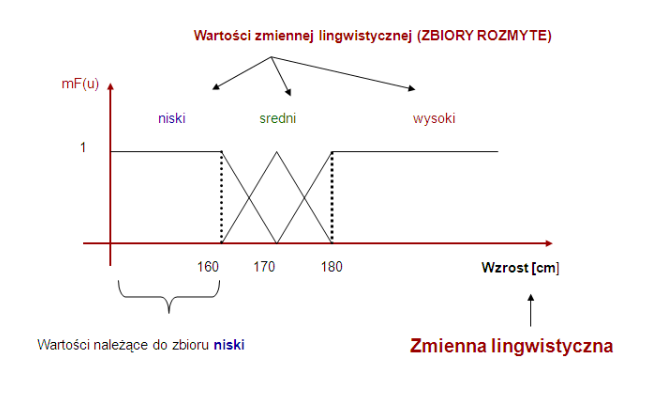
\includegraphics[width=0.9\textwidth]{{Rysunki/FunkcjaPrzynaleznosci.png}}
	\caption{Przykład funkcji przynależności - trójkątnej oraz trapezoidalnej [3]}
\end{figure}


Wyjaśnijmy także, czym jest lingwistyczne podsumowanie. Niech \(\mathcal{D}\) będzie bazą danych składającą się z \(m\)
krotek opisujących poszczególne rekordy. Przyjmijmy, że każda kolumna opisuje cechę pewnego typu. Taką cechę możemy nazwać \emph{zmienną lingwistyczną}. Może ona przyjmować konkretne wartości liczbowe lub rozmyte (np. mało/trochę/dużo/sporo). Zdefiniujmy także \(P\). Niech \(P\) będzie podmiotem podsumowania lingwistycznego (np. mężczyźni, kobiety, samochody, zawodnicy). Bardzo ważnym elementem, wykorzystywanym we wszystkich rodzajach podsumowań
lingwistycznych, jest kwantyfikator oznaczany jako \(Q\).
Przykładami kwantyfikatorów mogą być: "około 10", "ponad 70"
(kwantyfikatory absolutne - zbiory rozmyte na uniwersum \(\mathbb{R}\)) lub "większość", "znikoma część"
(kwantyfikatory relatywne - zbiory rozmyte na uniwersum \([0,\, 1]\)). Istotny dla nas będzie stopień przynależności \(P\) do \(Q\). Zdefiniujmy także sumaryzator \(S_j\). Jest to zbiór rozmyty na zbiorze wartości przyjmowanych przez \(j\)-tą kolumnę bazy danych. Np. gdyby krotki dotyczyły różnych pojazdów, a jedną ze zmiennych lingwistycznych
była ich prędkość, to sumaryzatory mogłyby mieć postać "jeździ szybko","jeździ ponad 200km/h" itp.

\vspace\baselineskip

Wykorzystując powyższe elementy można skonstruować \textbf{lingwistyczne podsumowanie
bazy danych}, czyli:
\[Q ~ P \mbox{ jest/są } S_j ~[T] ~\mbox{,}\]
gdzie \(T\) to stopień prawdziwości podsumowania.

\vspace\baselineskip

Przykład : \emph{Dużo studentów zarabia średnią krajową [0.64]}, gdzie: "dużo" to kwantyfikator, "studentów" to podmit lingwistyczny, "zarabia średnią krajową" to sumaryztaor, a "[0,64]" to stopień prawdziwości podsumowania. \newline

W celu rozszerzenie podsumowania lingwistycznego należy skorzystać ze złożonego sumaryztora. Sumę sumaryzatorów można w podsumowaniu lingwistycznym zapisać
za pomocą słowa "lub", zaś iloczyn za pomocą słowa "i".
W rezultacie \textbf{podsumowanie ze złożonym sumaryzatorem} może
mieć postać:
\[Q ~ P \mbox{ jest/są } S_1 \mbox{ i/lub } S_2 \mbox{ i/lub } \ldots \mbox{ i/lub } S_n  ~[T] ~\mbox{.}\]

\vspace\baselineskip

Przykład: \emph{Dużo studentów zarabia średnią krajową i/lub nosi okulary [0.44]}. \newline

Innym sposobem rozszerzenia pojęcia podsumowań
jest zastosowanie kwalifikatora. Kwalifikator
\(W\) jest zbiorem rozmytym na \(\mathcal{D}\),
który opisuje jakąś dodatkową właściwość. Typowe przykłady to "[osoby] które są bezrobotne",
"[osoby] które są dziećmi". \textbf{Podsumowanie
z~kwalifikatorem} ma postać:
\[Q ~ P \mbox{ mających własność } W \mbox{ ma własność } S_j ~[T] ~\mbox{.}\]

\vspace\baselineskip

Przykład: \emph{Studenci, którzy mają blond włosy zarabiają średnią krajową [028]}.\newline

Aby określić jakość naszych podsumowaniań zaimplementowaliśmy poniższe miary jakości:

\subsection{\(T_1\) -- stopień prawdziwości}

Stopień prawdziwości jest najbardziej naturalną miarą jakości podsumowania. Określa ona sumę przynależności wszystkich rozważanych krotek do sumaryzatora \(S_j\):
\[r = \sum_{i=1}^{m} \mu_{\mathrm{ce}(S_j)}(d_i) ~\mbox{,}\]
gdzie \(\mathrm{ce}(S_j)\) jest rozszerzeniem cylindrycznym
sumaryzatora \(S_j\), \(m\) liczba wszystkich krotek, a \(d_i\).
Dla kwantyfikatorów relatywnych stopnień
prawdziwości możemy zapisać jako
$$T_1 = \mu_Q(\frac{r}{m}),$$
zaś dla kwantyfikatorów absolutnych jako
$$T_1 = \mu_Q(r),$$
gdzie \(r\) jest kardynalnością. 

\subsection{\(T_2\) -- stopień nieprecyzyjności}
Dla podsumowania z \(n\) sumaryzatorami \(S_1 \ldots S_n\) możemy określić stopień nieprecyzyjności,
definiowany następującym wzorem:
\[T_2 = 1 - \left(\prod_{j=1}^{n} \mathrm{in}(S_j)\right)^{1/n} ~\mbox{.}\]
Wyrażenie \(\left(\prod_{j=1}^{n} \mathrm{in}(S_j)\right)^{1/n}\) to określa średnią geometryczna ze stopni rozmycia wykorzystanych sumaryzatorów, czyli w jakim stopniu precyzyjny jest sumaryzator. Im mniejszy nośnik zbioru rozmytego, tym wyższa jest jego precyzja.
   

\subsection{\(T_3\) -- stopień pokrycia}
Stopień pokrycia \(T_3\) jest zdefiniowany dla podsumowań z kwalifikatorami. Stopień pokrycia T3 
Dla każdego \(i=1\ldots m\) (związanego z krotką \(d_i\) z bazy
danych) możemy zdefiniować (z kwalifikatorem):
\[
\begin{array}{l}
t_i = \begin{cases}
1 & \mbox{gdy } \mu_{\mathrm{ce}(S_j)}(d_i) > 0 ~ \wedge ~ \mu_{W}(d_i) > 0 \\
0 & \mbox{w przeciwnym wypadku.}
\end{cases} \\
h_i = \begin{cases}
1 & \mbox{gdy } \mu_{W}(d_i) > 0 \\
0 & \mbox{w przeciwnym wypadku.}
\end{cases}
\end{array}\]

Bez kwalifikatora:

\[
\begin{array}{l}
t_i = \begin{cases}
1 & \mbox{gdy } \mu_{\mathrm{ce}(S_j)}(d_i) > 0  \\
0 & \mbox{w przeciwnym wypadku.}
\end{cases} \\
\end{array}\]

Przy powyższych oznaczeniach:
\[T_3 = \frac{\sum_{i=1}^{m} t_i}{\sum_{i=1}^{m} h_i} ~\mbox{.}\]

Reprezentuje stopień w jakim nośnik sumaryzatora pokrywa się z nośnikiem kwalifikatora.


\subsection{\(T_4\) -- stopień trafności}
Dla podsumowania z \(n\) sumaryzatorami \(S_1 \ldots S_n\)
oraz \(m\) krotkami w bazie danych możemy wprowadzić oznaczenia:
\[g_{ij} = \begin{cases}
1 & \mbox{gdy } \mu_{\mathrm{ce}(S_j)}(d_i) > 0 \\
0 & \mbox{w przeciwnym wypadku.}
\end{cases}\]
oraz
\[r_j = \frac{\sum_{i=1}^{m} g_{ij}}{m} ~\mbox{.}\]
Wówczas możemy zapisać:
\[T_4 = \left| \prod_{j=1}^{n} r_j - T_3\right| ~\mbox{.}\]

 Określa jak wiele krotek przynależy do sumaryzatora, czyli czy dane podsumowanie jest właściwe dla zestawu danych.

\subsection{\(T_5\) -- długość podsumowania}
Dla podsumowania z \(n\) sumaryzatorami \(S_1 \ldots S_n\)
miarę długości podsumowania definiujemy jako:
\[T_5 =  2 \left(\frac{1}{2}\right)^{|s|} ~\mbox{.}\]

Gdzie \(|s|\) jest ilością zbiorów rozmytych,z  których skomponowany jest sumaryzator. Określa jakość podsumowania na podstawie złożoności sumaryzatora, czyli im więcej składowych sumaryzatora złożonego, tym niższa wartość tej miary.

\subsection{\(T_6\) -- stopień nieprecyzyjności kwantyfikatora}
\(T_6\), czyli stopień nieprecyzyjności kwantyfikatora możemy zdefiniować jako:

\[T_6 = 1-\mathrm{in}(Q) ~\mbox{.}\]

Reprezentuje w jakim stopniu precyzyjny jest kwantyfikator. Im mniejszy nośnik zbioru rozmytego tym wyższa jest jego precyzja.

\subsection{\(T_7\) -- stopień liczności kwantyfikatora}
W przeciwieństwie do \(T_6\), zamiast zliczać elementy z nośnika \(Q\),
policzymy moc zbioru rozmytego:
\[T_7 = 1-\frac{|Q|}{|\mathcal{X}_Q|} ~\mbox{.}\]

Opisuje stopień precyzji kwantyfikatora, im mniejsza kardynalność kwantyfikatora tym jest on bardziej precyzyjny.

\subsection{\(T_8\) -- stopień liczności sumaryzatora}
W przypadku zastosowania sumaryzatora złożonego, podobnie jak przy poprzednich miarach, stosujemy średnią geometryczną.
Dla podsumowania z \(n\) sumaryzatorami \(S_1 \ldots S_n\):

\[T_8 = 1- \left(\prod_{j=1}^{n} \frac{|S_j|}{|\mathcal{X}_j|}\right)^{\frac{1}{n}} ~\mbox{.}\]

Opisuje stopień precyzji sumaryzatora, im mniejsza kardynalność kwantyfikatora tym jest on bardziej precyzyjny.

\subsection{\(T_9\) -- stopień nieprecyzyjności kwalifikatora}
Stopień precyzji kwalifikatora \(T_9\) jest oparty na drugiej formie podsumowań tzn.: Q obiektów będących/mających W jest/ma S, gdzie W jest reprezentowane przez zbiór rozmyty i jest kwalifikatorem. Definicja tej miary jest następująca:
\[T_9 = 1-\mathrm{in}(W) ~\mbox{.}\]

Określa w jakim stopniu precyzyjny jest kwalifikator. Im szerszy nośnik zbioru rozmytego tym niższa jest jego precyzja, gdyż bierze pod uwagę większy zakres wartości. 


\subsection{\(T_{10}\) -- stopień liczności kwalifikatora}
Stopień kardynalności kwalifikatora \(T_{10}\) definiujemy jako:
\[T_{10} = 1-\frac{|W|}{|\mathcal{X}_g|} ~\mbox{.}\]\\

Opisuje stopień precyzji kwalifikatora, im większa jest kardynalność kwalifikator tym jest on mniej precyzyjny.

\subsection{\(T_{11}\) -- długość kwalifikatora}
Długość kwalifikatora \(T_{11}\) definiujemy następująco:
\[T_{11} = 2\left(\frac{1}{2}\right)^{|W|} ~\mbox{.}\]

Wyznacza jakość podsumowania na podstawie złożoności kwalifikatora, Im bardziej złożony kwalifikator tym jakość podsumowania gorsza.

\vspace\baselineskip

\section{Opis implementacji}
Program został stworzony w języku C\#. Graficzny interfejs użytkownika został stworzony przy  wykorzystaniu Windows Presentation Foundation. Logika aplikacji została odseparowana od GUI. W związku z tym, zaimplementowaliśmy trzy projekty: Logic, ViewModel oraz GUI.

\subsection{Logic}
W tym projekcie zawarta została cała logika aplikacji. Odzworowany został model naszej bazy danych (\emph{FifaPlayer.cs}), zaimplementowane zostały: funkcje przynależności trójkątna (\emph{TriangularFunction.cs}) oraz trapezoidalna (\emph{TrapezoidFunction}), zmienna lingwistyczna (\emph{LinguisticVariable.cs}), kwantyfikator (\emph{Quantifier.cs}), zmienna, która "na sztywno" określa nasz kwantyfikator (np. słaby, przeciętny, dobry) w zależności od podanych danych (\emph{Variable.cs}), sumaryzator "i" (\emph{And.cs}), a także sumaryzator "lub" (\emph{Or.cs}). W projekcie logic znajduje się takża klasa (\emph{Measures.cs}), gdzie zawarliśmy wszystkie 11 miar jakości podsumowań.
 
\subsection{ViewModel}

Klasa MainViewModel przyjmuje dane wejściowe od użytkownika i reaguje na jego poczynania wywołując wybrane akcje z logiki programu oraz odpowiada za odświeżanie widoków w interfejsie graficznym.

\subsection{GUI}

Projekt GUI (graphical user interface) implementuje przejrzysty oraz łatwy w obsłudze graficzny interfejs użytkownika.

\section{Materiały i metody}

\subsection{Baza danych}
Do przeprowadzenia badań i generowania konkretnych podsumowań wykorzystaliśmy bazę danych dotyczącą przechowującą statystyki piłkarzy z gry Fifa 2019 [4].Składa się ona z 15397 krotek znajdujących się w tabeli z 20 różnymi kolumnami - w ramach naszego projektu skorzystaliśmy z 13. Przedstawiamy je poniżej:

\begin{itemize}
	\item Wiek - wartości z przedziału [17-45]
	\item Wzrost (cm) - wartości z przedziału [155-205]
	\item Waga (kg) - wartości z przedziału [50-11] 
	\item Tempo - wartości z przedziału [0-97]
	\item Przyspieszenie - wartości z przedziału [13-98]
	\item Prędkość - wartości z przedziału [12-97]
	\item Dribbling - wartości z przedziału [0-97]
	\item Zręczność - wartości z przedziału [14-98]
	\item Balans - wartości z przedziału [16-99]
	\item Reakcje - wartości z przedziału [30-96]
	\item Kontrola piłki - wartości z przedziału [3-97]
	\item Opanowanie - wartości z przedziału [3-97]
	\item Precyzja - wartości z przedziału [0-93]
	\item Ustawienie się - wartości z przedziału [2-95]
\end{itemize}

Każda z ww. kolumn jest typem całkowitym.

\subsection{Sumaryzatory i kwalifikatory}
Poniżej zaprezentowaliśmy poszczególne sumaryzatory oraz kwalifikatory wykorzystane w naszym programie. 

\begin{table}[H]
	\centering
	\begin{tabular}{c c c c c} 
		\hline
		\textbf{Etykieta} & \textbf{a} & \textbf{b} & \textbf{c} &  \textbf{d} \\ [0.5ex] 
		\hline
		\hline 
		Bardzo młody & 17 & 17 & 18 & 20 \\ 
		Młody & 19 & 21 & 24 & 29 \\
		Dorosły & 28 & 30 & 35 & 37 \\
		Dojrzały & 36 & 40 & 45 & 45\\
		\hline
	\end{tabular}
	\caption{Przyporządkowane parametry funkcji trapezoidalnej dla wieku.}
\end{table}

\begin{table}[H]
	\centering
	\begin{tabular}{c c c c c} 
		\hline
		\textbf{Etykieta} & \textbf{a} & \textbf{b} & \textbf{c} &  \textbf{d} \\ [0.5ex] 
		\hline
		\hline 
		Bardzo niski & 155 & 155 & 160 & 162 \\ 
		Niski & 161 & 165 & 168 & 170 \\
		Przeciętny & 169 & 172 & 176 & 180 \\
		Wysoki & 179 & 182 & 186 & 192\\
		Bardzo wysoki & 191 & 196 & 205 & 205\\
		\hline
	\end{tabular}
	\caption{Przyporządkowane parametry funkcji trapezoidalnej dla wzrostu.}
\end{table}

\begin{table}[H]
	\centering
	\begin{tabular}{c c c c c} 
		\hline
		\textbf{Etykieta} & \textbf{a} & \textbf{b} & \textbf{c} &  \textbf{d} \\ [0.5ex] 
		\hline
		\hline 
		Niska & 50 & 59 & 66 & 73 \\ 
		Standardowa & 72 & 77 & 79 & 84 \\
		Postawna & 83 & 86 & 89 & 91 \\
		Ciężka & 90 & 98 & 110 & 110\\
		\hline
	\end{tabular}
	\caption{Przyporządkowane parametry funkcji trapezoidalnej dla wzrostu.}
\end{table}

\begin{table}[H]
	\centering
	\begin{tabular}{c c c c c} 
		\hline
		\textbf{Etykieta} & \textbf{a} & \textbf{b} & \textbf{c} &  \textbf{d} \\ [0.5ex] 
		\hline
		\hline 
		Niskie & 0 & 15 & 27 & 35 \\ 
		Średnie & 33 & 46 & 58 & 66 \\
		Wysokie & 65 & 79 & 88 & 97 \\
		\hline
	\end{tabular}
	\caption{Przyporządkowane parametry funkcji trapezoidalnej dla tempa.}
\end{table}

\begin{table}[H]
	\centering
	\begin{tabular}{c c c c c} 
		\hline
		\textbf{Etykieta} & \textbf{a} & \textbf{b} & \textbf{c} &  \textbf{d} \\ [0.5ex] 
		\hline
		\hline 
		Słabe & 13 & 25 & 29 & 35 \\ 
		Przeciętne & 33 & 46 & 58 & 66 \\
		Dobre & 65 & 79 & 88 & 98 \\
		\hline
	\end{tabular}
	\caption{Przyporządkowane parametry funkcji trapezoidalnej dla przyspieszenia.}
\end{table}

\begin{table}[H]
	\centering
	\begin{tabular}{c c c c c} 
		\hline
		\textbf{Etykieta} & \textbf{a} & \textbf{b} & \textbf{c} &  \textbf{d} \\ [0.5ex] 
		\hline
		\hline 
		Słaba & 12 & 25 & 29 & 35 \\ 
		Przeciętna & 33 & 46 & 58 & 69 \\
		Dobra & 65 & 79 & 88 & 97 \\
		\hline
	\end{tabular}
	\caption{Przyporządkowane parametry funkcji trapezoidalnej dla prędkości.}
\end{table}

\begin{table}[H]
	\centering
	\begin{tabular}{c c c c c} 
		\hline
		\textbf{Etykieta} & \textbf{a} & \textbf{b} & \textbf{c} &  \textbf{d} \\ [0.5ex] 
		\hline
		\hline 
		Słaby & 0 & 15 & 27 & 37 \\ 
		Przeciętny & 36 & 46 & 58 & 66 \\
		Dobry & 67 & 79 & 88 & 97 \\
		\hline
	\end{tabular}
	\caption{Przyporządkowane parametry funkcji trapezoidalnej dla dribblingu.}
\end{table}

\begin{table}[H]
	\centering
	\begin{tabular}{c c c c c} 
		\hline
		\textbf{Etykieta} & \textbf{a} & \textbf{b} & \textbf{c} &  \textbf{d} \\ [0.5ex] 
		\hline
		\hline 
		Słaba & 14 & 21 & 27 & 35 \\ 
		Przeciętna & 33 & 46 & 58 & 69 \\
		Dobra & 67 & 79 & 88 & 98 \\
		\hline
	\end{tabular}
	\caption{Przyporządkowane parametry funkcji trapezoidalnej dla zręczności.}
\end{table}

\begin{table}[H]
	\centering
	\begin{tabular}{c c c c c} 
		\hline
		\textbf{Etykieta} & \textbf{a} & \textbf{b} & \textbf{c} &  \textbf{d} \\ [0.5ex] 
		\hline
		\hline 
		Słaby & 16 & 21 & 29 & 35 \\ 
		Przeciętny & 38 & 46 & 58 & 72 \\
		Dobry & 71 & 79 & 88 & 99 \\
		\hline
	\end{tabular}
	\caption{Przyporządkowane parametry funkcji trapezoidalnej dla balansu.}
\end{table}

\begin{table}[H]
	\centering
	\begin{tabular}{c c c c c} 
		\hline
		\textbf{Etykieta} & \textbf{a} & \textbf{b} & \textbf{c} &  \textbf{d} \\ [0.5ex] 
		\hline
		\hline 
		Słabe & 30 & 37 & 43 & 47 \\ 
		Przeciętne & 46 & 59 & 66 & 72 \\
		Szybkie & 71 & 79 & 88 & 96 \\
		\hline
	\end{tabular}
	\caption{Przyporządkowane parametry funkcji trapezoidalnej dla reakcji.}
\end{table}

\begin{table}[H]
	\centering
	\begin{tabular}{c c c c c} 
		\hline
		\textbf{Etykieta} & \textbf{a} & \textbf{b} & \textbf{c} &  \textbf{d} \\ [0.5ex] 
		\hline
		\hline 
		Słaba & 3 & 14 & 23 & 26 \\ 
		Przeciętna & 25 & 39 & 48 & 57 \\
		Dobra & 56 & 63 & 69 & 75 \\
		Bardzo dobra & 74 & 81 & 88 & 99 \\
		\hline
	\end{tabular}
	\caption{Przyporządkowane parametry funkcji trapezoidalnej dla kontroli piłki.}
\end{table}

\begin{table}[H]
	\centering
	\begin{tabular}{c c c c c} 
		\hline
		\textbf{Etykieta} & \textbf{a} & \textbf{b} & \textbf{c} &  \textbf{d} \\ [0.5ex] 
		\hline
		\hline 
		Słabe & 3 & 15 & 24 & 32 \\ 
		Zadowalające & 31 & 44 & 57 & 66 \\
		Bardzo dobre & 65 & 75 & 88 & 97 \\
		\hline
	\end{tabular}
	\caption{Przyporządkowane parametry funkcji trapezoidalnej dla opanowania.}
\end{table}

\begin{table}[H]
	\centering
	\begin{tabular}{c c c c c} 
		\hline
		\textbf{Etykieta} & \textbf{a} & \textbf{b} & \textbf{c} &  \textbf{d} \\ [0.5ex] 
		\hline
		\hline 
		Słaba & 3 & 15 & 24 & 32 \\ 
		Przeciętna & 31 & 44 & 57 & 66 \\
		Dobra & 65 & 75 & 88 & 97 \\
		\hline
	\end{tabular}
	\caption{Przyporządkowane parametry funkcji trapezoidalnej dla celności.}
\end{table}

\begin{table}[H]
	\centering
	\begin{tabular}{c c c c c} 
		\hline
		\textbf{Etykieta} & \textbf{a} & \textbf{b} & \textbf{c} &  \textbf{d} \\ [0.5ex] 
		\hline
		\hline 
		Słabe & 3 & 15 & 24 & 32 \\ 
		Przeciętne & 31 & 44 & 57 & 66 \\
		Dobre & 65 & 75 & 88 & 97 \\
		\hline
	\end{tabular}
	\caption{Przyporządkowane parametry funkcji trapezoidalnej dla ustawiania się.}
\end{table}

\subsection{Kwantyfikatory}
Kwantyfikatory podzieliliśmy na względne i absolutne . Przedstawiamy je poniżej:

\begin{table}[H]
	\centering
	\begin{tabular}{c c c c c c} 
		\hline
		\textbf{Etykieta} & \textbf{Funkcja przynależności} & \textbf{a} & \textbf{b} & \textbf{c} &  \textbf{d} \\ [0.5ex] 
		\hline
		\hline 
		Żaden & Trójkątna & 0 & 0 & 0.1 & - \\ 
		Mniej niż ćwierć & Trapezoidalna & 0 & 0 & 0.25 & 0.35 \\
		Około jedna trzecia & Trójkątna & 0.23 & 0.33 & 0.43 & - \\
		Około połowa & Trójkątna & 0.4 & 0.5 & 0.6 & - \\
		Około dwie trzecie & Trójkątna & 0.56 & 0.66 & 0.76 & - \\
		Większość & Trójkątna & 0.73 & 0.83 & 0.93 & - \\
		Prawie każdy & Trójkątna & 0.85 & 0.9 & 1.05 & - \\
		\hline
	\end{tabular}
	\caption{Przyporządkowane parametry dla kwantyfikatora względnego.}
\end{table}
\begin{table}[H]
	\centering
	\begin{tabular}{c c c c c c} 
		\hline
		\textbf{Etykieta} & \textbf{Funkcja przynależności} & \textbf{a} & \textbf{b} & \textbf{c} &  \textbf{d} \\ [0.5ex] 
		\hline
		\hline 
		Mniej niż 100 & Trapezoidalna & 0 & 0 & 99 & 150 \\ 
		Około 250 & Trójkątna & 150 & 250 & 350 & - \\
		Około 500 & Trójkątna & 400 & 500 & 600 & - \\
		Około 750 & Trójkątna & 650 & 750 & 850 & - \\
		Więcej niż 100 & Trapezoidalna & 950 & 1000 & 15397 & 15397 \\
		\hline
	\end{tabular}
	\caption{Przyporządkowane parametry dla kwantyfikatora absolutnego.}
\end{table}




\section{Badania}

Postanowiliśmy podzielić nasze badania na 3 części:
\begin{enumerate}
	\item W pierwszym badaniu sprawdzaliśmy jakie wartości przybiorą miary podsumowań dla różnych kwantyfikatorów.
	\item W drugim teście porównywaliśmy podsumowania z oraz bez kwalifikatora.
	\item W trzecim badaniu naszym celem było porównanie podsumowań z jednym sumaryzatorem oraz ich połączeń spójnikami ORAZ i LUB.
\end{enumerate}

\subsection{Pierwszy eksperyment}

W tym badaniu wygenerowaliśmy 3 komunikaty, dotyczące odpowiednio zależności pomiędzy:
\begin{enumerate}
	\item Dobrą Celnością a Przeciętnym Ustawianiem się,
	\item Słabą Prędkością a Zadowalającym Opanowaniem,
	\item Młodym Wiekiem a Dobrą Prędkością.
\end{enumerate}
Miary $T2-T5$ oraz $T8-T11$ były stałe, dlatego nie umieszczaliśmy ich w tabeli oraz na wykresie, gdyż kwantyfikator nie miał wpływu na ich wartość. Zamieściliśmy ich wartości pod tabelą porównującą wartości miar $T1$, $T6$ i $T7$. 

\subsubsection{Eksperyment 1.1}

\begin{figure}[H]
	\centering
	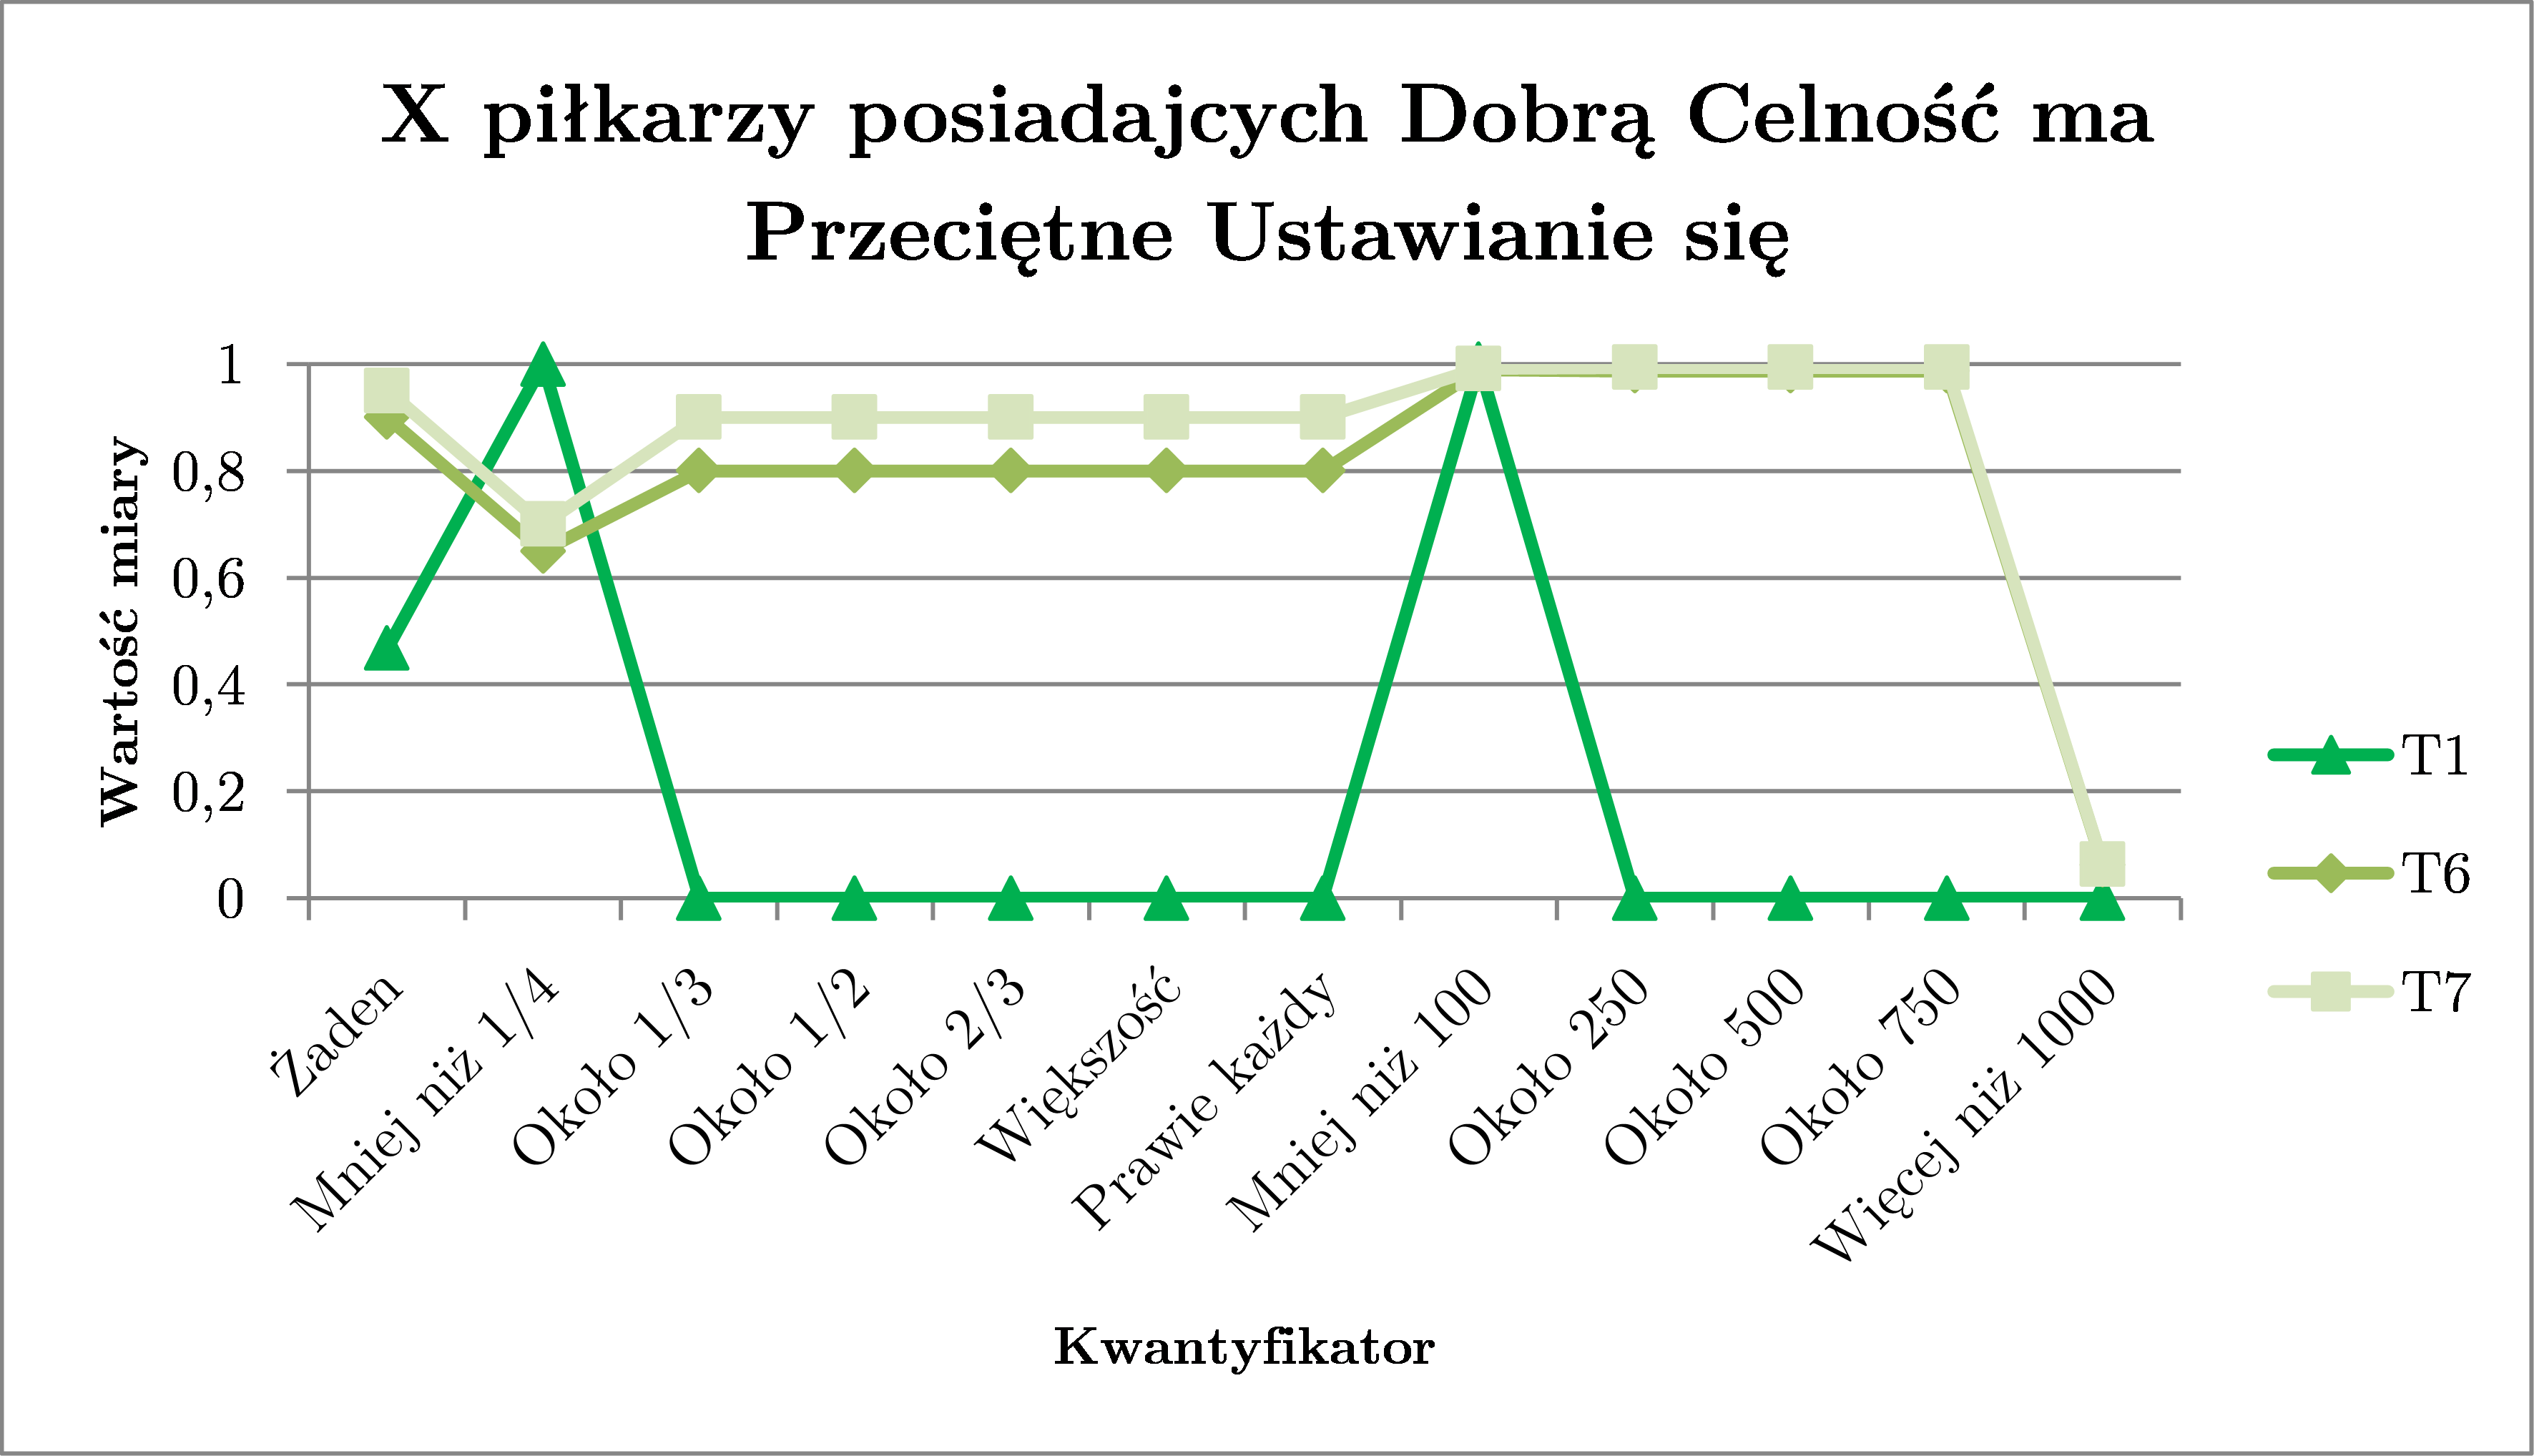
\includegraphics[width=0.9\textwidth]{{Rysunki/Badanie11.png}}
	\caption{Wykres przedstawiający wyniki Eksperymentu 1.1}
\end{figure}

\begin{table}[H]
	\centering
	\begin{tabular}{c c c c c c} 
		\hline
		\textbf{Kwantyfikator} & \textbf{T1} & \textbf{T6} & \textbf{T7}\\ [0.5ex] 
		\hline
		\hline 
		Żaden & 0.468 & 0.9 & 0.95 \\ 
		Mniej niż 1/4 & 1 & 0.65 & 0.7 \\
		Około 1/3 & 0 & 0.8 & 0.9 \\
		Około 1/2 & 0 & 0.8 & 0.9 \\
		Około 2/3 & 0 & 0.8 & 0.9 \\
		Większość & 0 & 0.8 & 0.9  \\
		Prawie każdy & 0 & 0.8 & 0.9  \\
		Mniej niż 100 & 1 & 0.99 & 0.992  \\
		Około 250 & 0 & 0.987 & 0.994  \\
		Około 500 & 0 & 0.987 & 0.994  \\
		Około 750 & 0 & 0.987 & 0.994  \\
		Więcej niż 1000 & 0 & 0.987 & 0.063  \\
		\hline
	\end{tabular}
	\caption{Tabela przedstawiający wyniki Eksperymentu 1.1}
\end{table}

Uzyskane miary, które były jednakowe dla każdego kwantyfikatora: $T2 = 0.431$, $T3 = 0.151$, $T4 = 0.263$, $T5 = 1$, $T8 = 0.998$, $T9 = 0.827$, $T10 = 0.999$, $T11 = 1$.

\subsubsection{Eksperyment 1.2}

\begin{figure}[H]
	\centering
	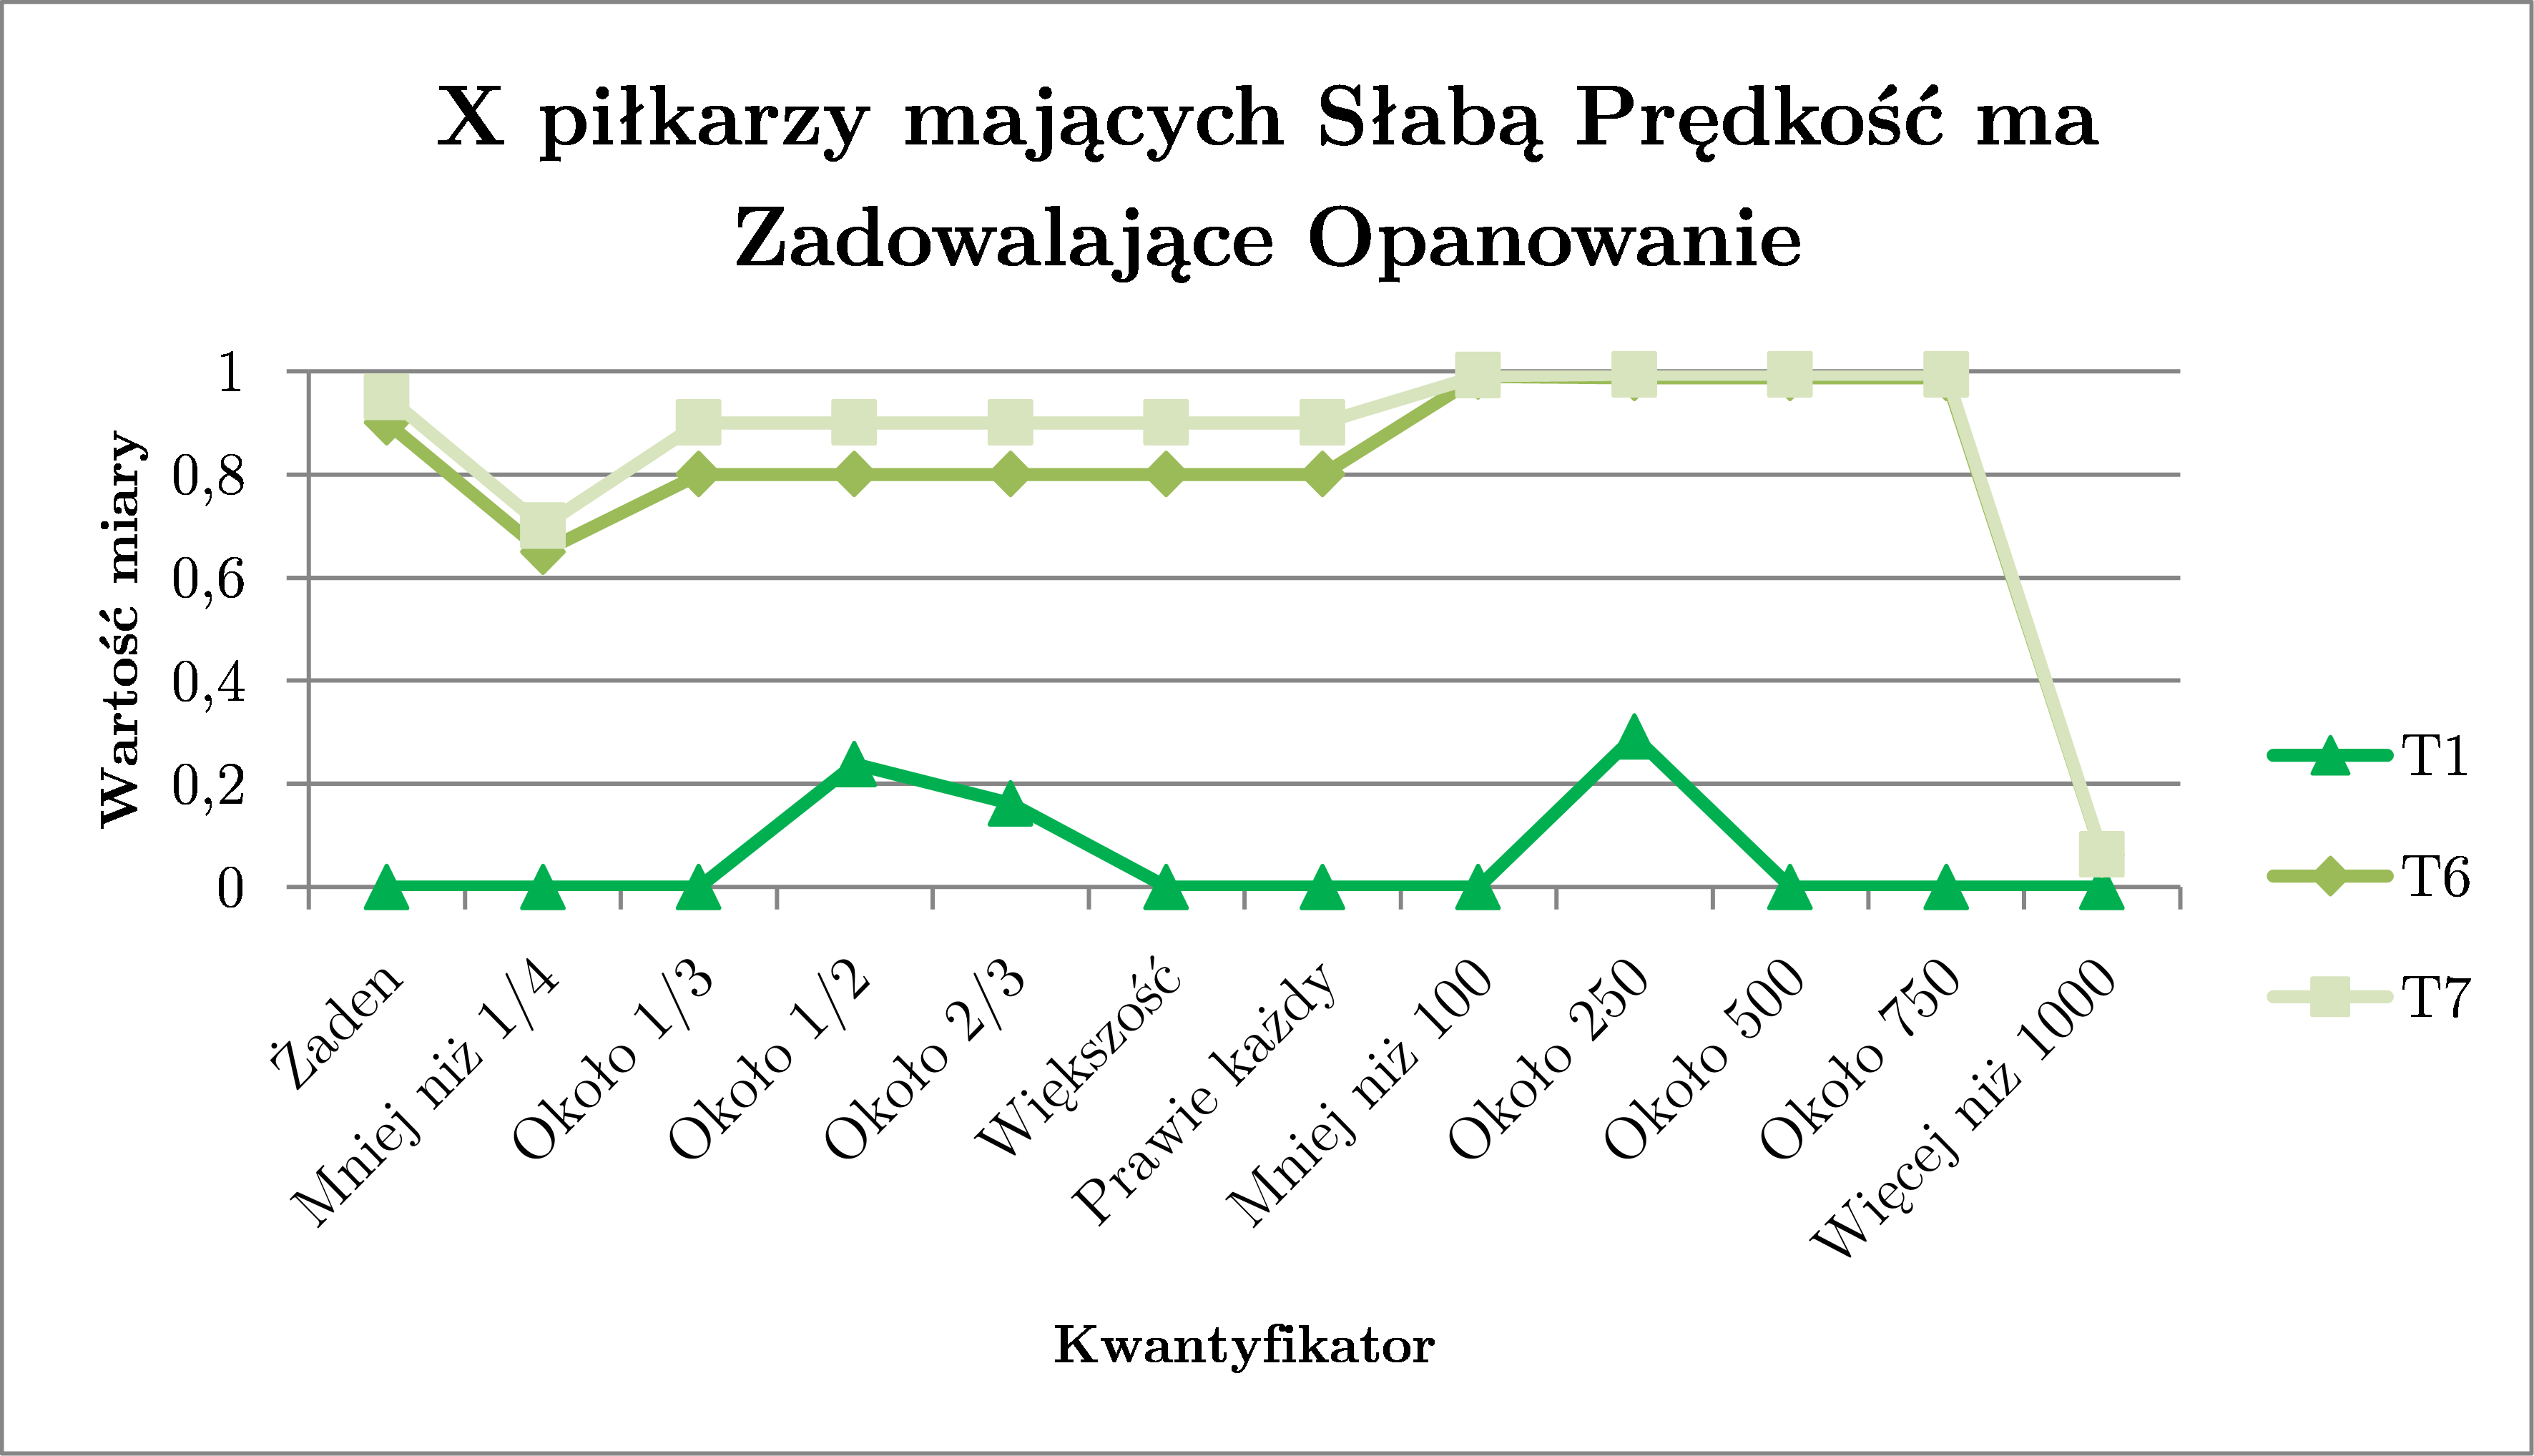
\includegraphics[width=0.9\textwidth]{{Rysunki/Badanie12.png}}
	\caption{Wykres przedstawiający wyniki Eksperymentu 1.2}
\end{figure}

\begin{table}[H]
	\centering
	\begin{tabular}{c c c c c c} 
		\hline
		\textbf{Kwantyfikator} & \textbf{T1} & \textbf{T6} & \textbf{T7}\\ [0.5ex] 
		\hline
		\hline 
		Żaden & 0 & 0.9 & 0.95 \\ 
		Mniej niż 1/4 & 0 & 0.65 & 0.7 \\
		Około 1/3 & 0 & 0.8 & 0.9 \\
		Około 1/2 & 0.238 & 0.8 & 0.9 \\
		Około 2/3 & 0.162 & 0.8 & 0.9 \\
		Większość & 0 & 0.8 & 0.9  \\
		Prawie każdy & 0 & 0.8 & 0.9  \\
		Mniej niż 100 & 0 & 0.99 & 0.992  \\
		Około 250 & 0.292 & 0.987 & 0.994  \\
		Około 500 & 0 & 0.987 & 0.994  \\
		Około 750 & 0 & 0.987 & 0.994  \\
		Więcej niż 1000 & 0 & 0.062 & 0.063  \\
		\hline
		\hline
	\end{tabular}
	\caption{Tabela przedstawiający wyniki Eksperymentu 1.2}
\end{table}

Uzyskane miary, które były jednakowe dla każdego kwantyfikatora: $T2 = 0.318$, $T3 = 0.718$, $T4 = 0.211$, $T5 = 1$, $T8 = 0.998$, $T9 = 0.939$, $T10 = 0.999$, $T11 = 1$.

\subsubsection{Eksperyment 1.3}

\begin{figure}[H]
	\centering
	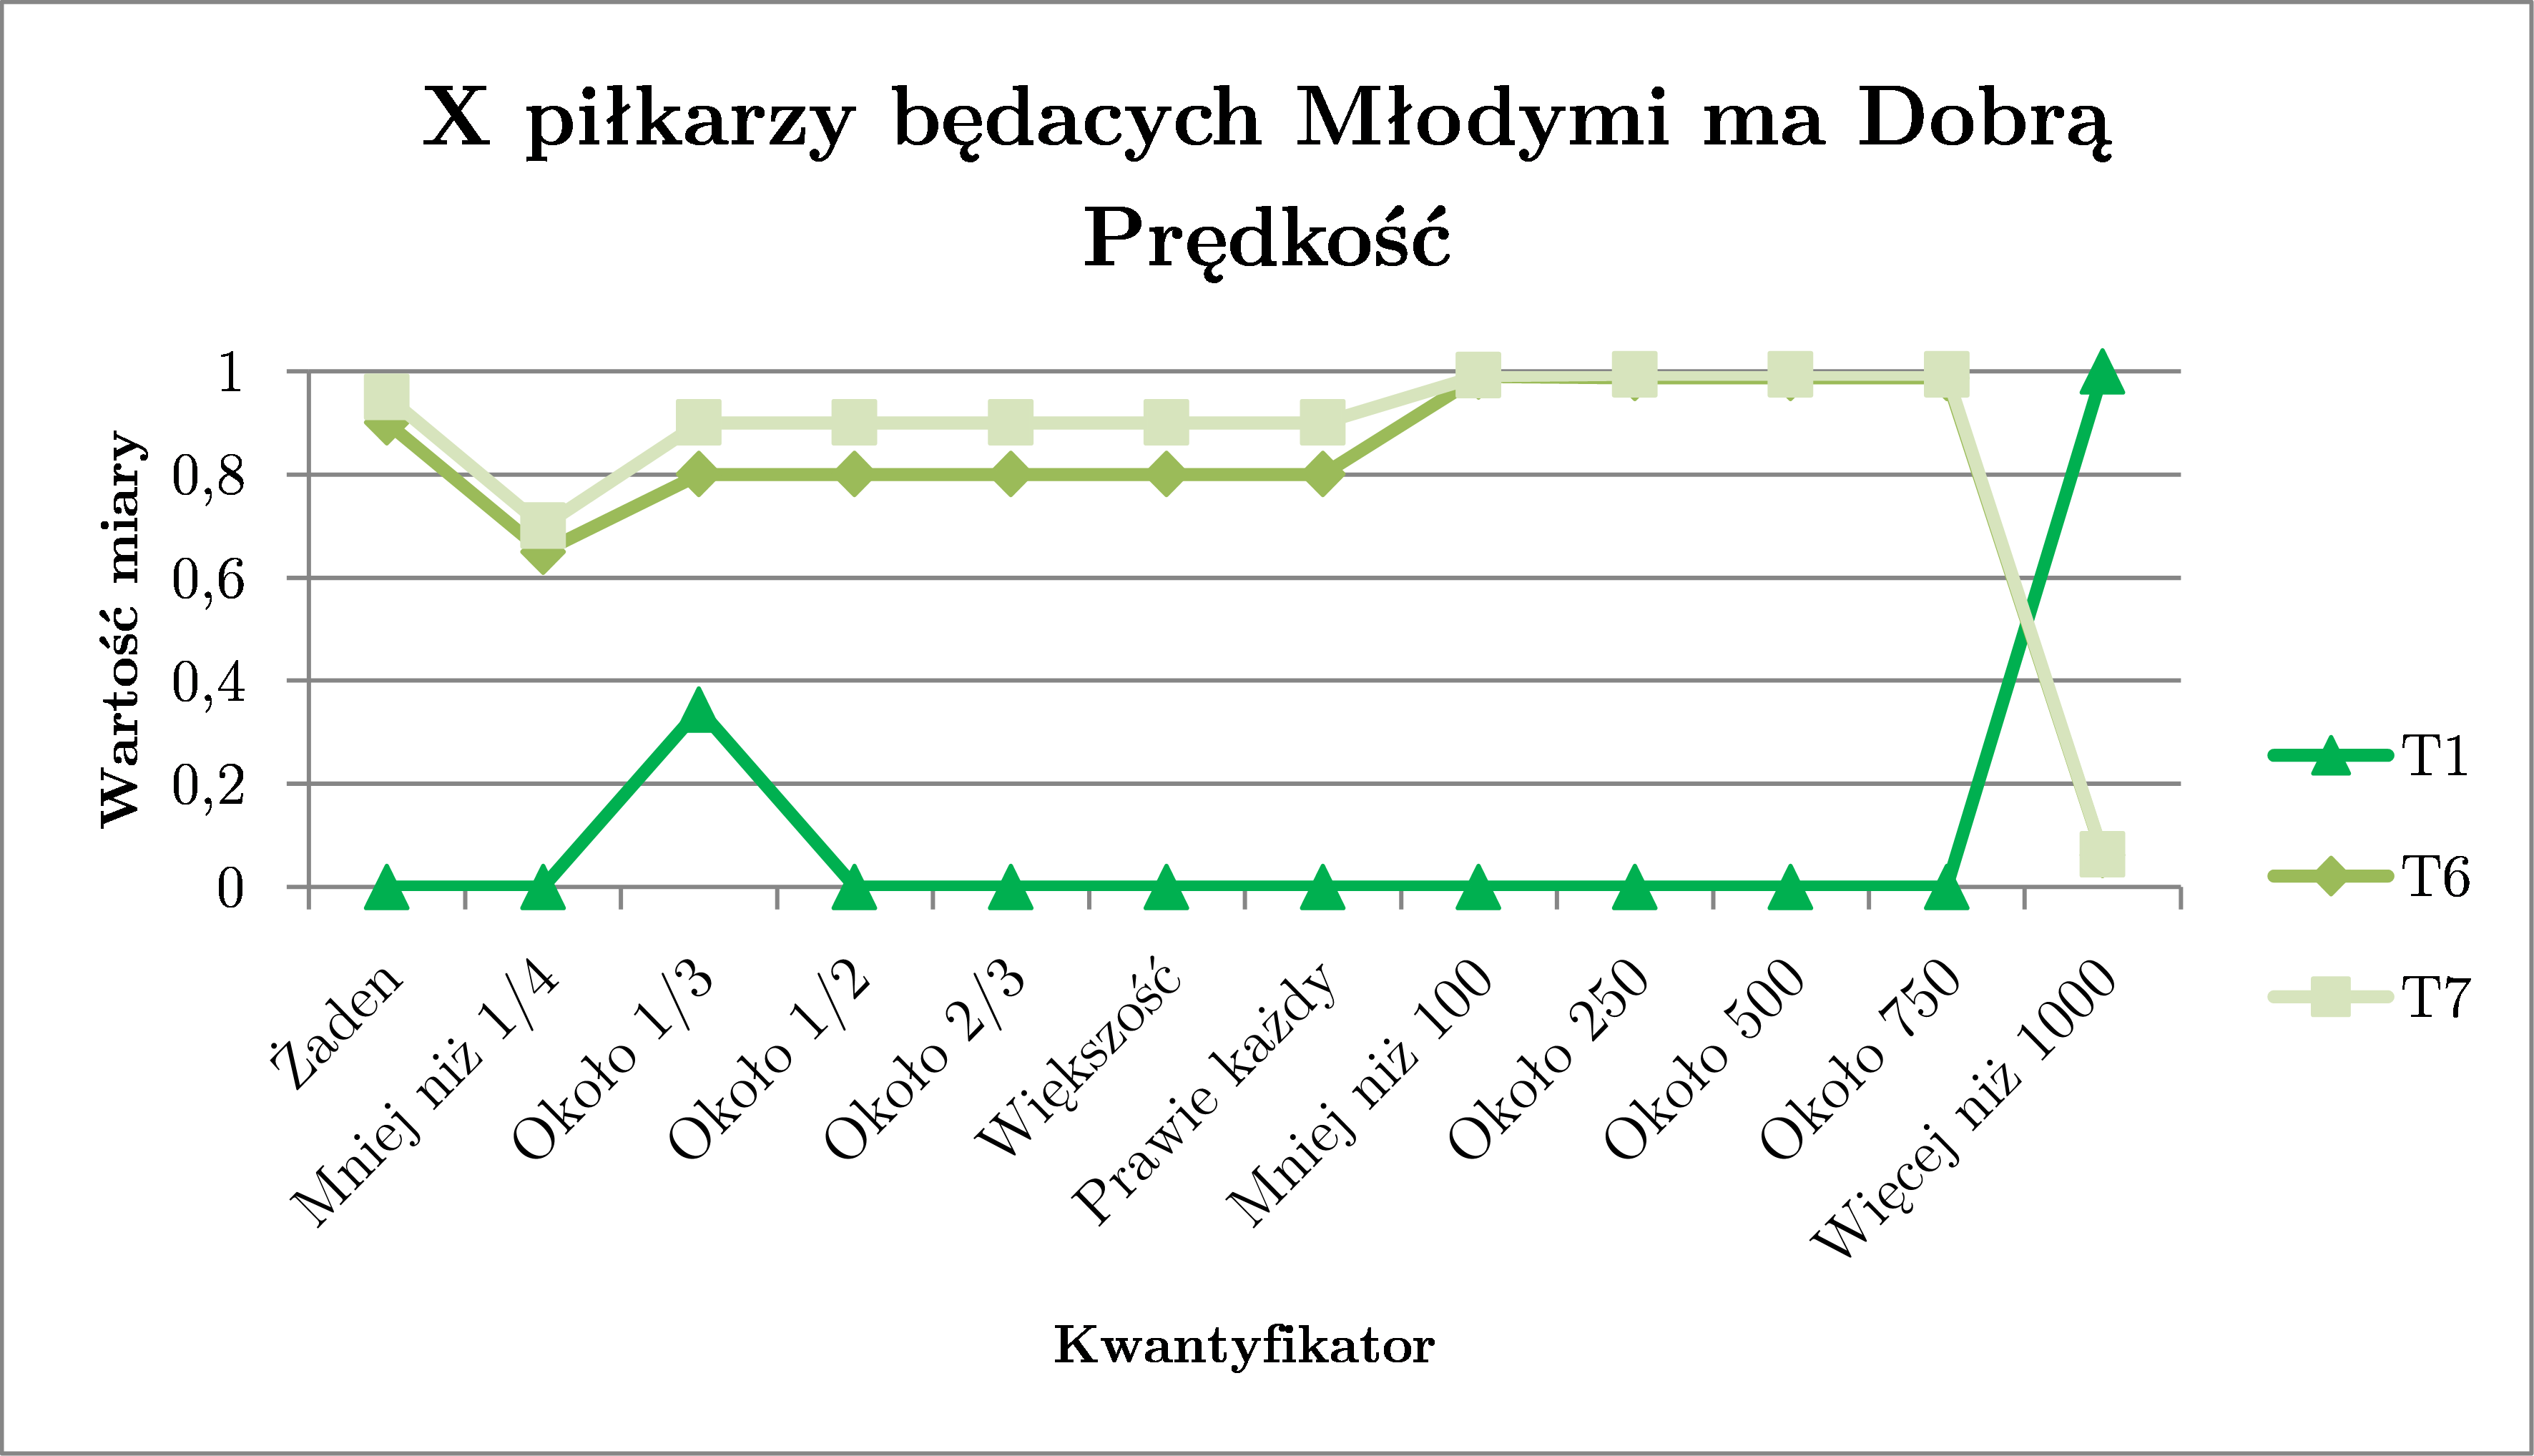
\includegraphics[width=0.9\textwidth]{{Rysunki/Badanie13.png}}
	\caption{Wykres przedstawiający wyniki Eksperymentu 1.3}
\end{figure}

\begin{table}[H]
	\centering
	\begin{tabular}{c c c c c c} 
		\hline
		\textbf{Kwantyfikator} & \textbf{T1} & \textbf{T6} & \textbf{T7}\\ [0.5ex] 
		\hline
		\hline 
		Żaden & 0 & 0.9 & 0.95 \\ 
		Mniej niż 1/4 & 0 & 0.65 & 0.7 \\
		Około 1/3 & 0.344 & 0.8 & 0.9 \\
		Około 1/2 & 0 & 0.8 & 0.9 \\
		Około 2/3 & 0 & 0.8 & 0.9 \\
		Większość & 0 & 0.8 & 0.9  \\
		Prawie każdy & 0 & 0.8 & 0.9  \\
		Mniej niż 100 & 0 & 0.99 & 0.992  \\
		Około 250 & 0 & 0.987 & 0.994  \\
		Około 500 & 0 & 0.987 & 0.994  \\
		Około 750 & 0 & 0.987 & 0.994  \\
		Więcej niż 1000 & 1 & 0.987 & 0.063  \\
		\hline
	\end{tabular}
	\caption{Tabela przedstawiający wyniki Eksperymentu 1.3}
\end{table}

Uzyskane miary, które były jednakowe dla każdego kwantyfikatora: $T2 = 0.499$, $T3 = 0.565$, $T4 = 0.254$, $T5 = 1$, $T8 = 0.999$, $T9 = 0.347$, $T10 = 1$, $T11 = 1$.

\subsection{Drugi eksperyment}

W tym badaniu wygenerowaliśmy 2 komunikaty, które skupiały się na:
\begin{enumerate}
	\item Przeciętnych Reakcjach,
	\item Standardowej Wadze.
\end{enumerate}
Porównywaliśmy wpływ obecności kwalifikatora (odpowiednio Słabego Bilansu oraz Niskiego Wzrostu) lub jego braku na wartości miar. Porównywaliśmy zarówno jednakowe jak i różniące się kwantyfikatory, tak, by miara T1 nie wynosiła 0.

\subsubsection{Eksperyment 2.1}

\begin{figure}[H]
	\centering
	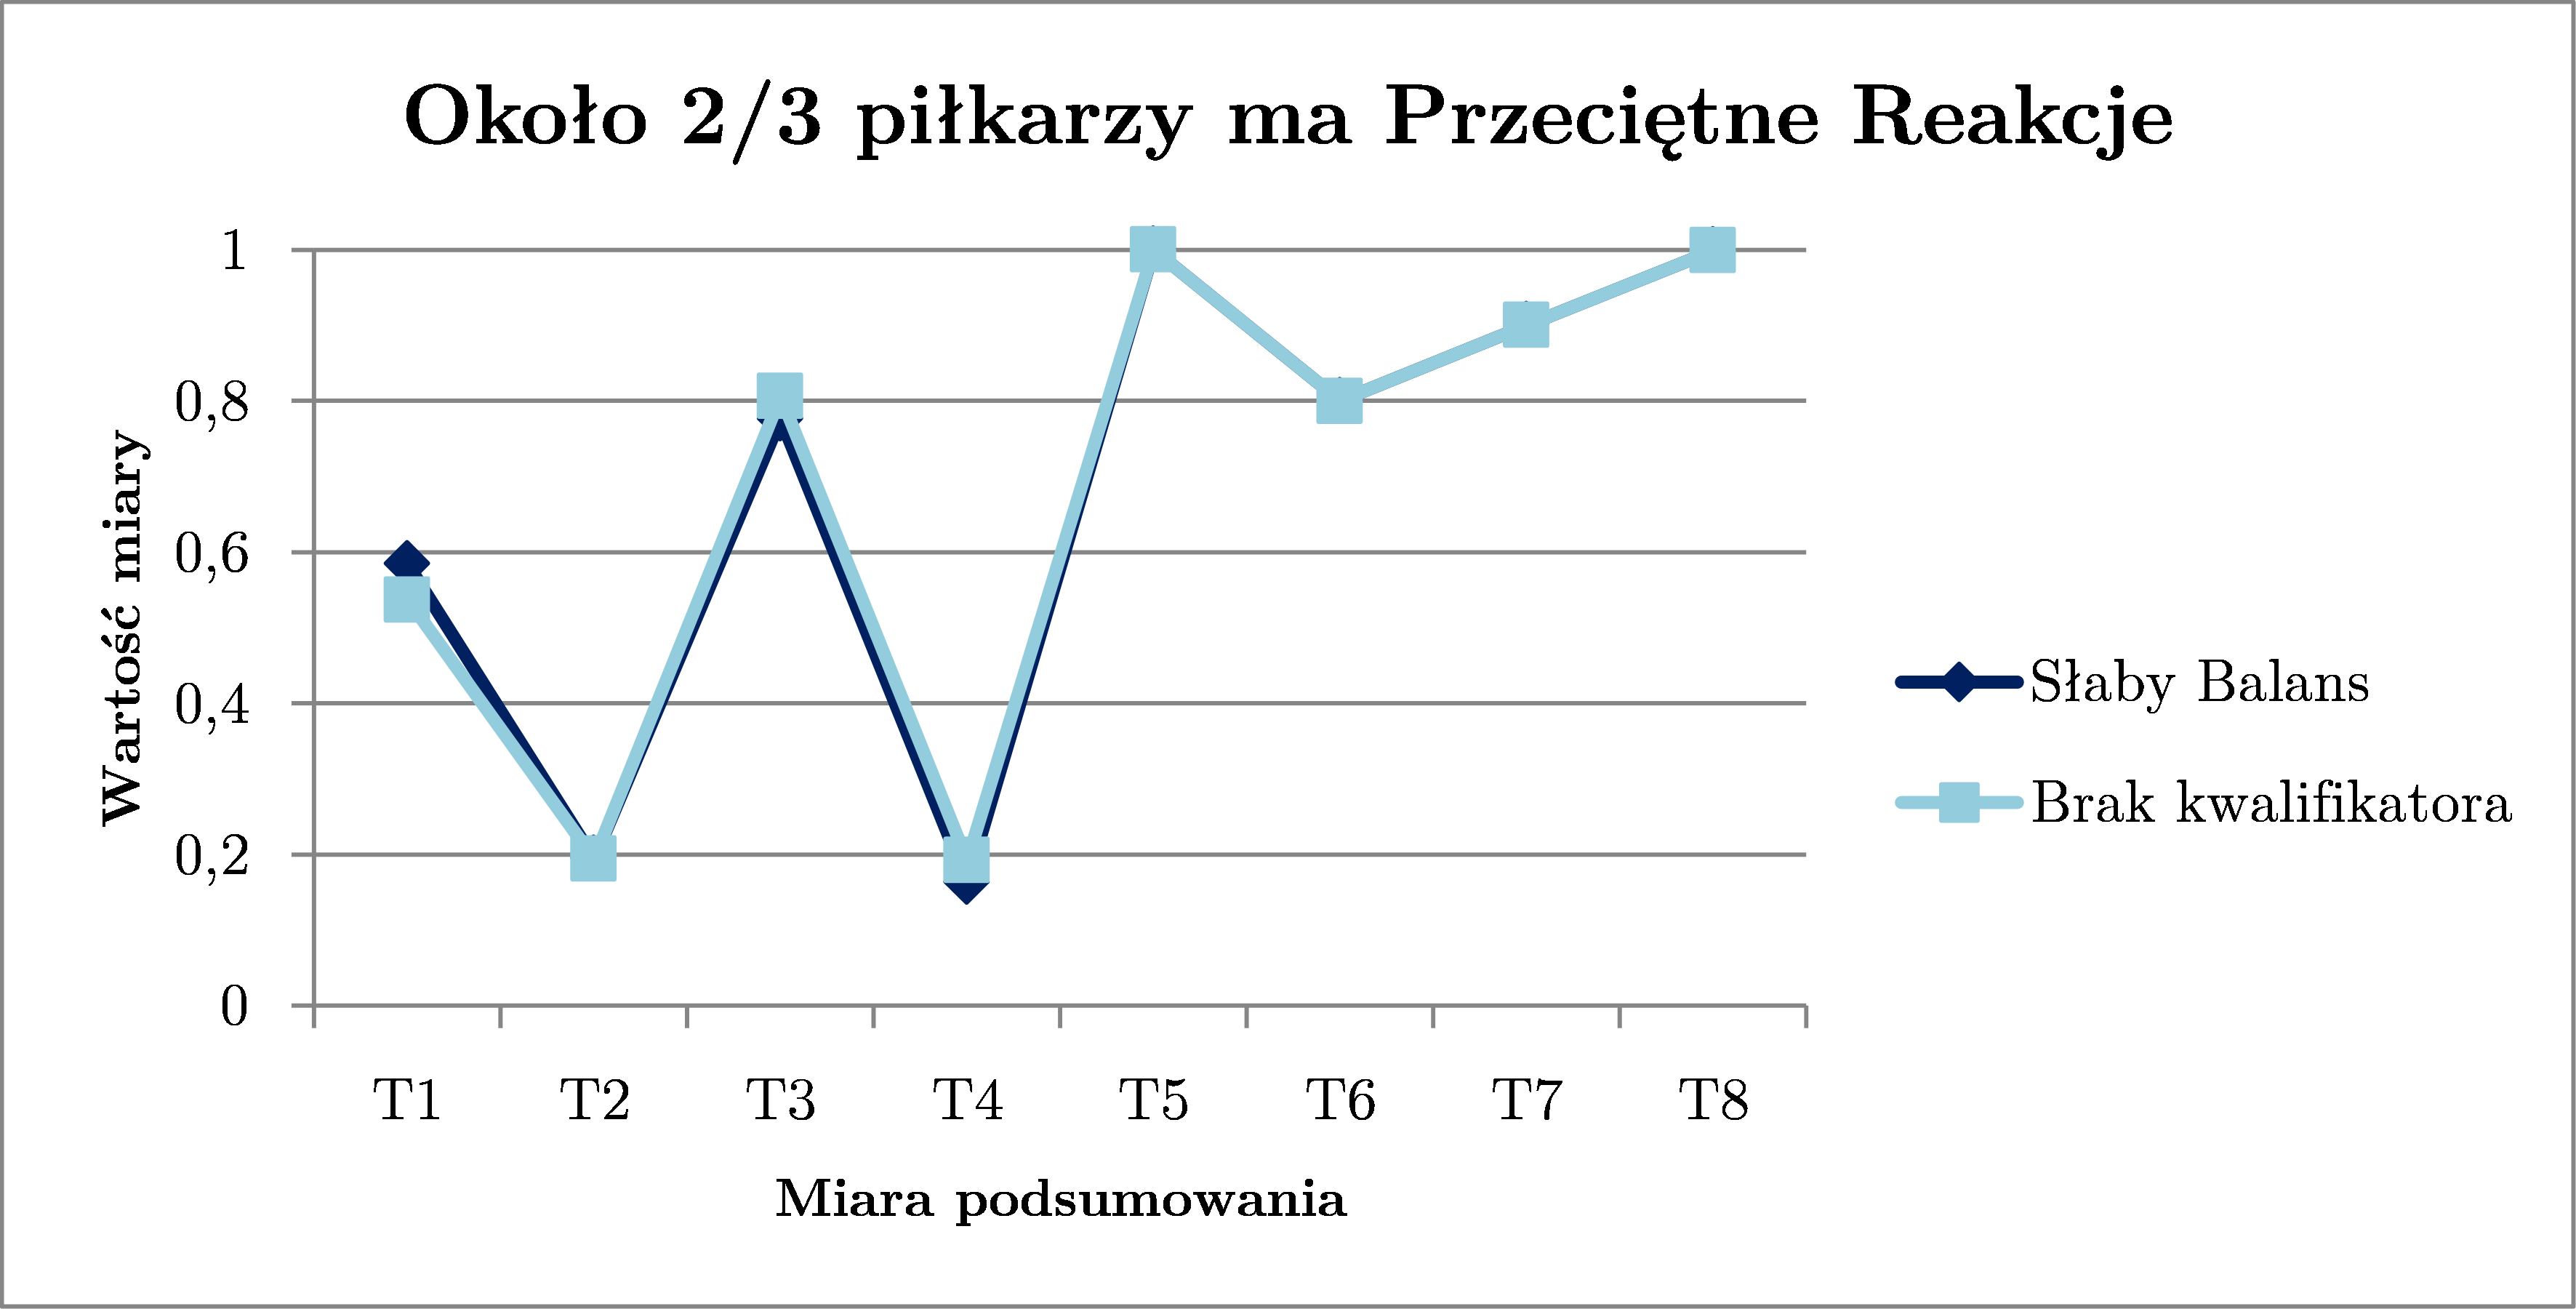
\includegraphics[width=0.9\textwidth]{{Rysunki/Badanie211.png}}
	\caption{Wykres przedstawiający wyniki Eksperymentu 2.1 - kwantyfikator względny}
\end{figure}

\begin{table}[H]
	\centering
	\begin{tabular}{c c c} 
		\hline
		\textbf{Miara} & \textbf{Słaby balans} & \textbf{Brak kwalifikatora}\\ [0.5ex] 
		\hline
		\hline 
		T1 & 0.584 & 0.537 \\
		T2 & 0.194 & 0.194 \\
		T3 & 0.776 & 0.806 \\
		T4 & 0.163 & 0.192 \\
		T5 & 1 & 1 \\
		T6 & 0.8 & 0.8 \\
		T7 & 0.9 & 0.9 \\
		T8 & 0.999 & 0.999 \\
		\hline
	\end{tabular}
	\caption{Tabela przedstawiająca wyniki Eksperymentu 2.1 - kwantyfikator względny (około 2/3 piłkarzy)}
\end{table}

\begin{figure}[H]
	\centering
	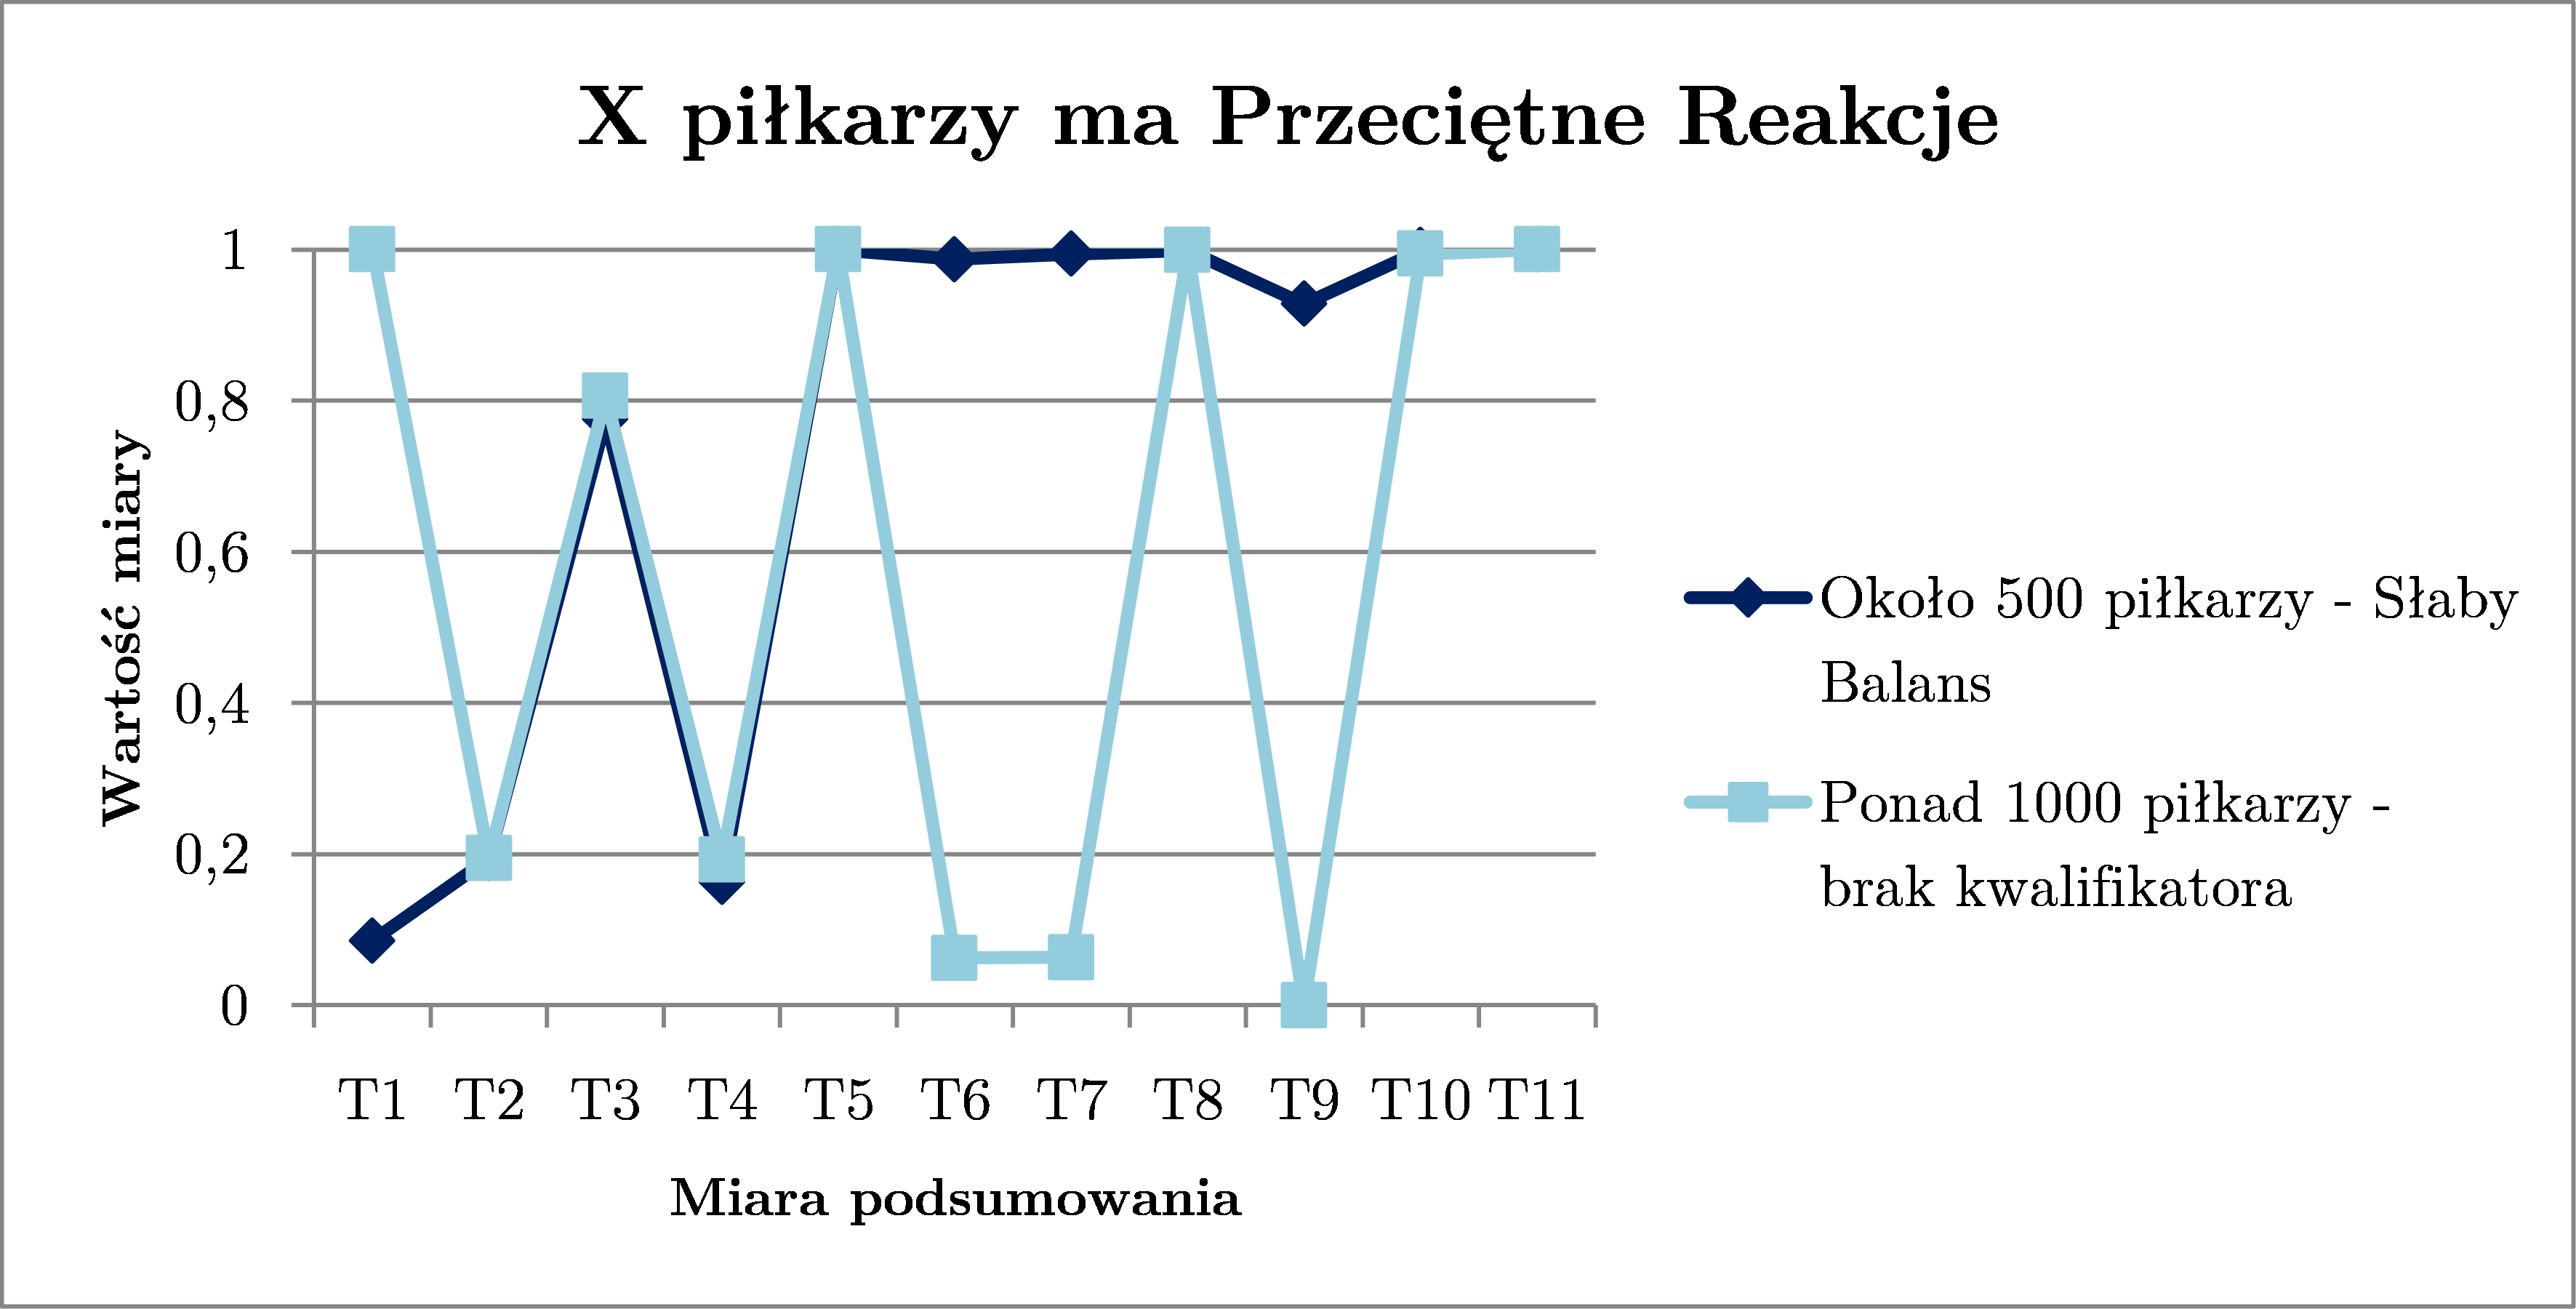
\includegraphics[width=0.9\textwidth]{{Rysunki/Badanie212.png}}
	\caption{Wykres przedstawiający wyniki Eksperymentu 2.1 - kwantyfikator bezwzględny}
\end{figure}

\begin{table}[H]
	\centering
	\begin{tabular}{c c c } 
		\hline
		& \textbf{Słaby balans} & \textbf{Brak kwalifikatora}\\ [0.5ex]
		\textbf{Miara} & \textbf{Około 500} & \textbf{Więcej niż 1000}\\ [0.5ex]
		\hline
		\hline 
		T1 & 0.537 & 1  \\
		T2 & 0.194 & 0.194 \\
		T3 & 0.776 & 0.806 \\
		T4 & 0.163 & 0.192 \\
		T5 & 1 & 1 \\
		T6 & 0.987 & 0.062 \\
		T7 & 0.994 & 0.063 \\
		T8 & 0.999 & 0.999 \\
		\hline
	\end{tabular}
	\caption{Tabela przedstawiająca wyniki Eksperymentu 2.1 - kwantyfikator bezwzględny}
\end{table}

\subsubsection{Eksperyment 2.2}

\begin{figure}[H]
	\centering
	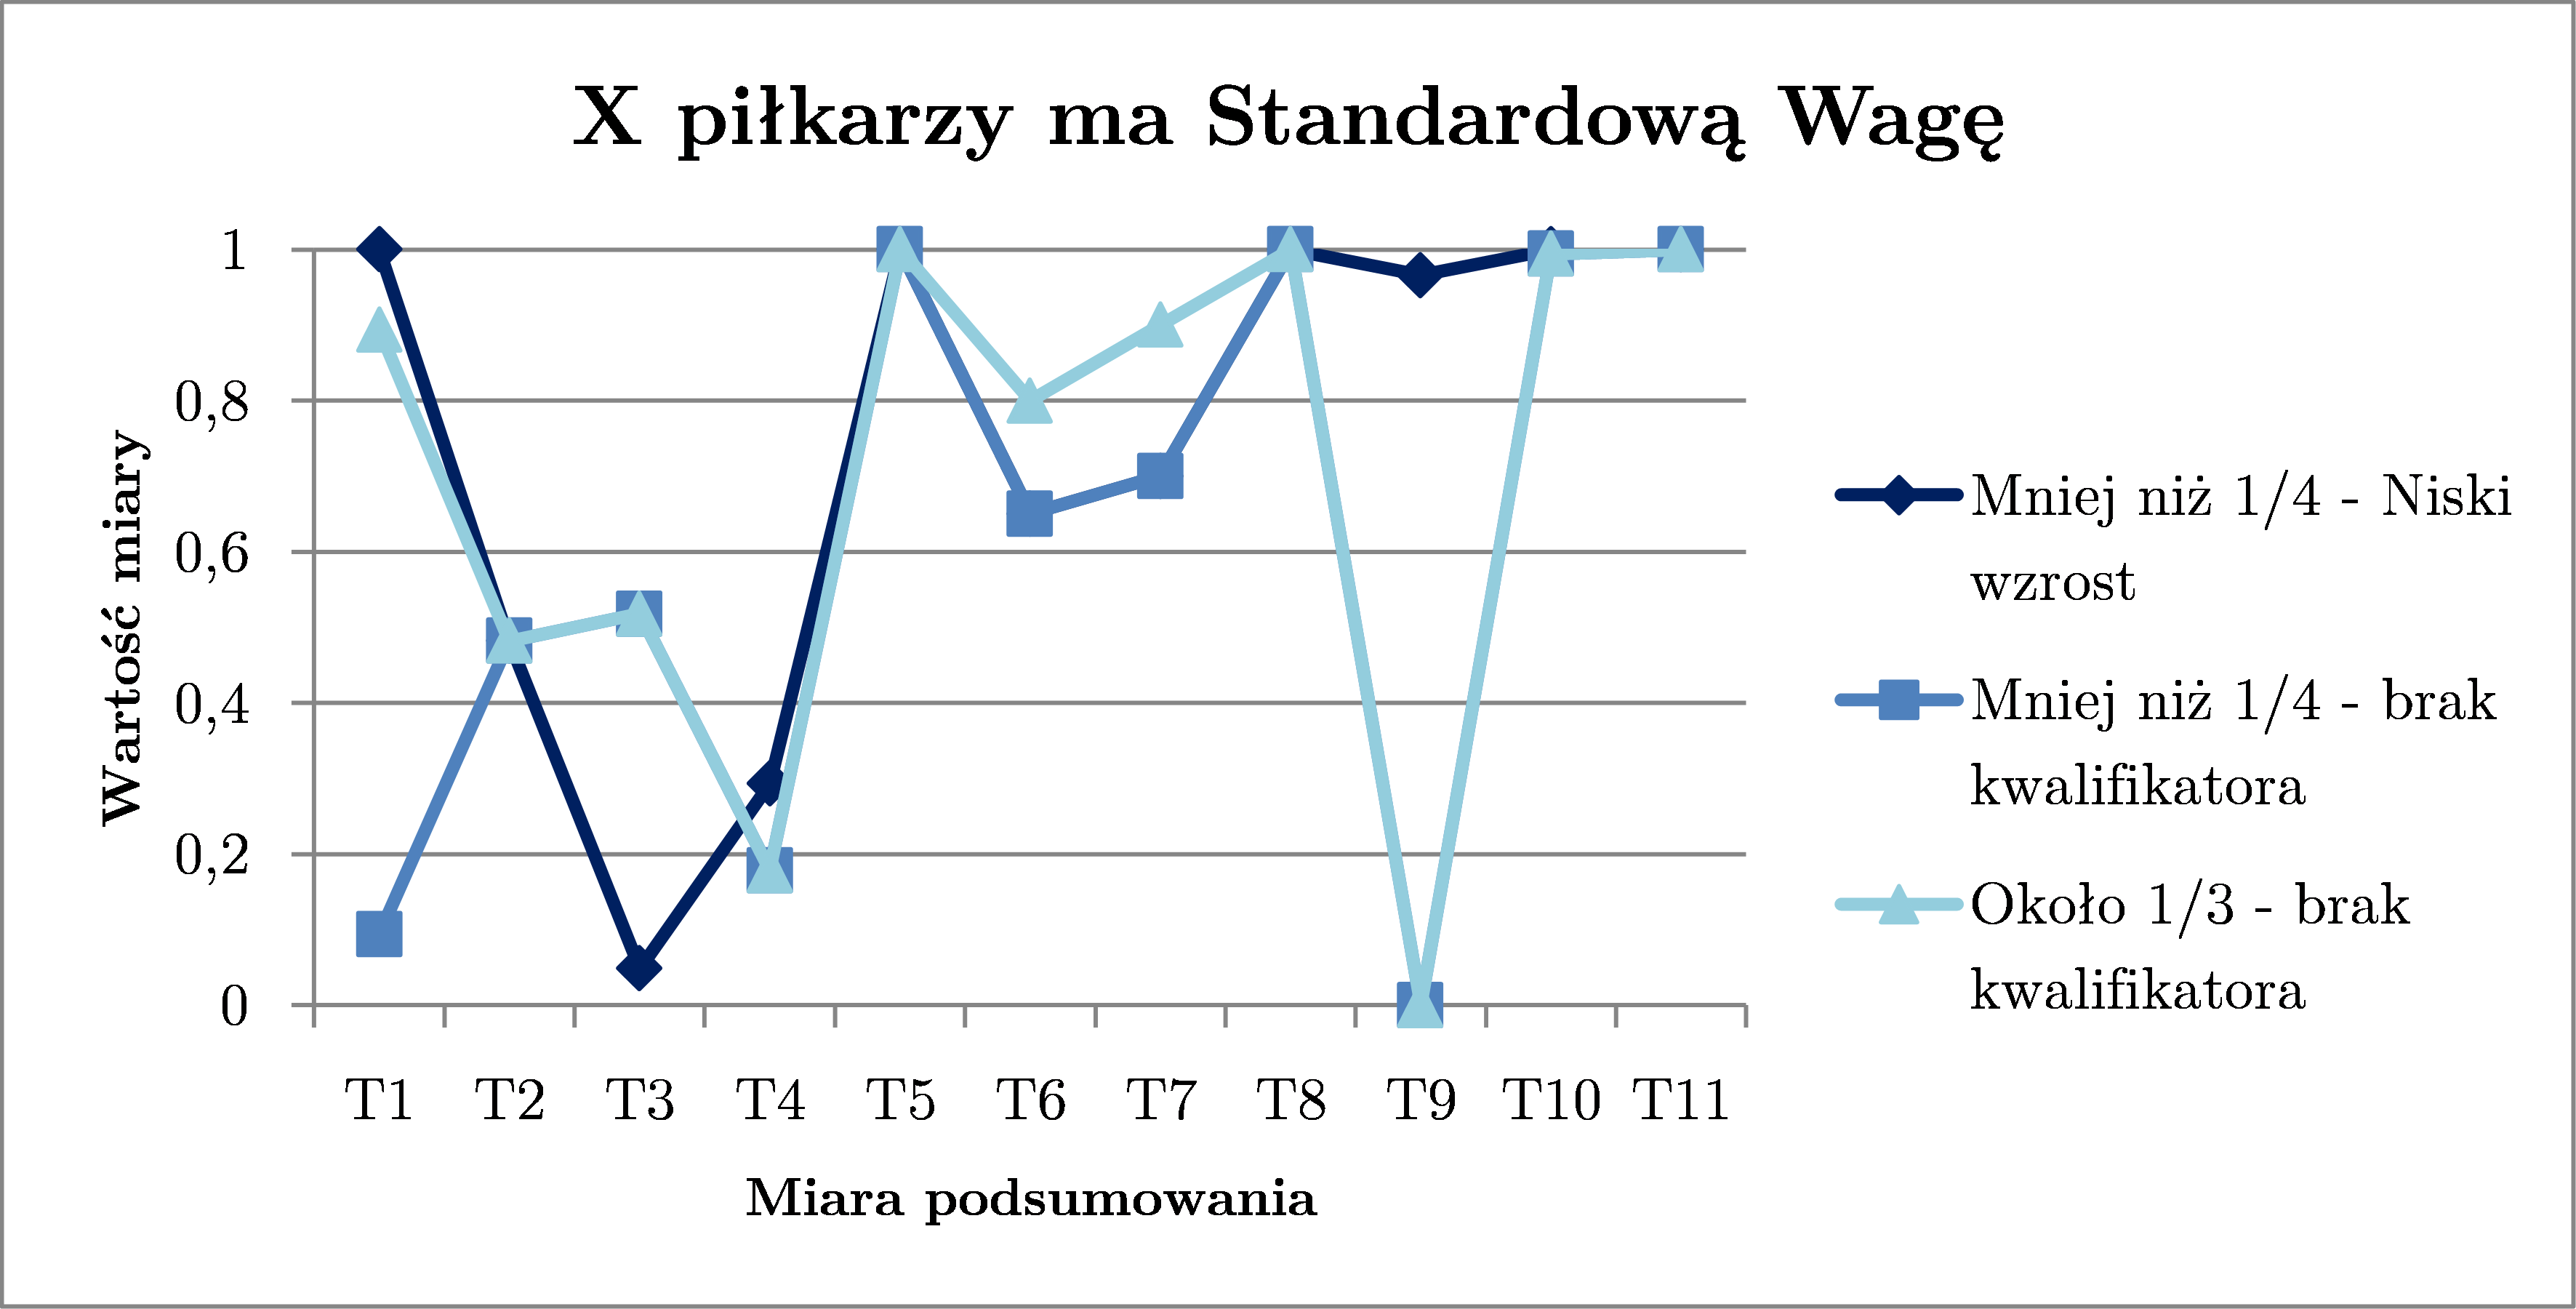
\includegraphics[width=0.9\textwidth]{{Rysunki/Badanie221.png}}
	\caption{Wykres przedstawiający wyniki Eksperymentu 2.2 - kwantyfikator względny}
\end{figure}

\begin{table}[H]
	\centering
	\begin{tabular}{c c c c } 
		\hline
		& \textbf{Niski Wzrost} & \textbf{Brak kwalifikatora} & \textbf{Brak kwalifikatora}\\ [0.5ex] 
		\textbf{Miara} & \textbf{Mniej niż 1/4} & \textbf{Mniej niż 1/4} & \textbf{1/3}\\ [0.5ex] 
		\hline
		\hline 
		T1 & 1 & 0.094 & 0.894 \\
		T2 & 0.482 & 0.482 & 0.482 \\
		T3 & 0.048 & 0.518 & 0.518 \\
		T4 & 0.293 & 0.178 & 0.178 \\
		T5 & 1 & 1 & 1 \\
		T6 & 0.65 & 0.65 & 0.8 \\
		T7 & 0.7 & 0.7 & 0.9 \\
		T8 & 1 & 1 & 1 \\
		\hline
	\end{tabular}
	\caption{Tabela przedstawiająca wyniki Eksperymentu 2.2 - kwantyfikator względny}
\end{table}

\begin{figure}[H]
	\centering
	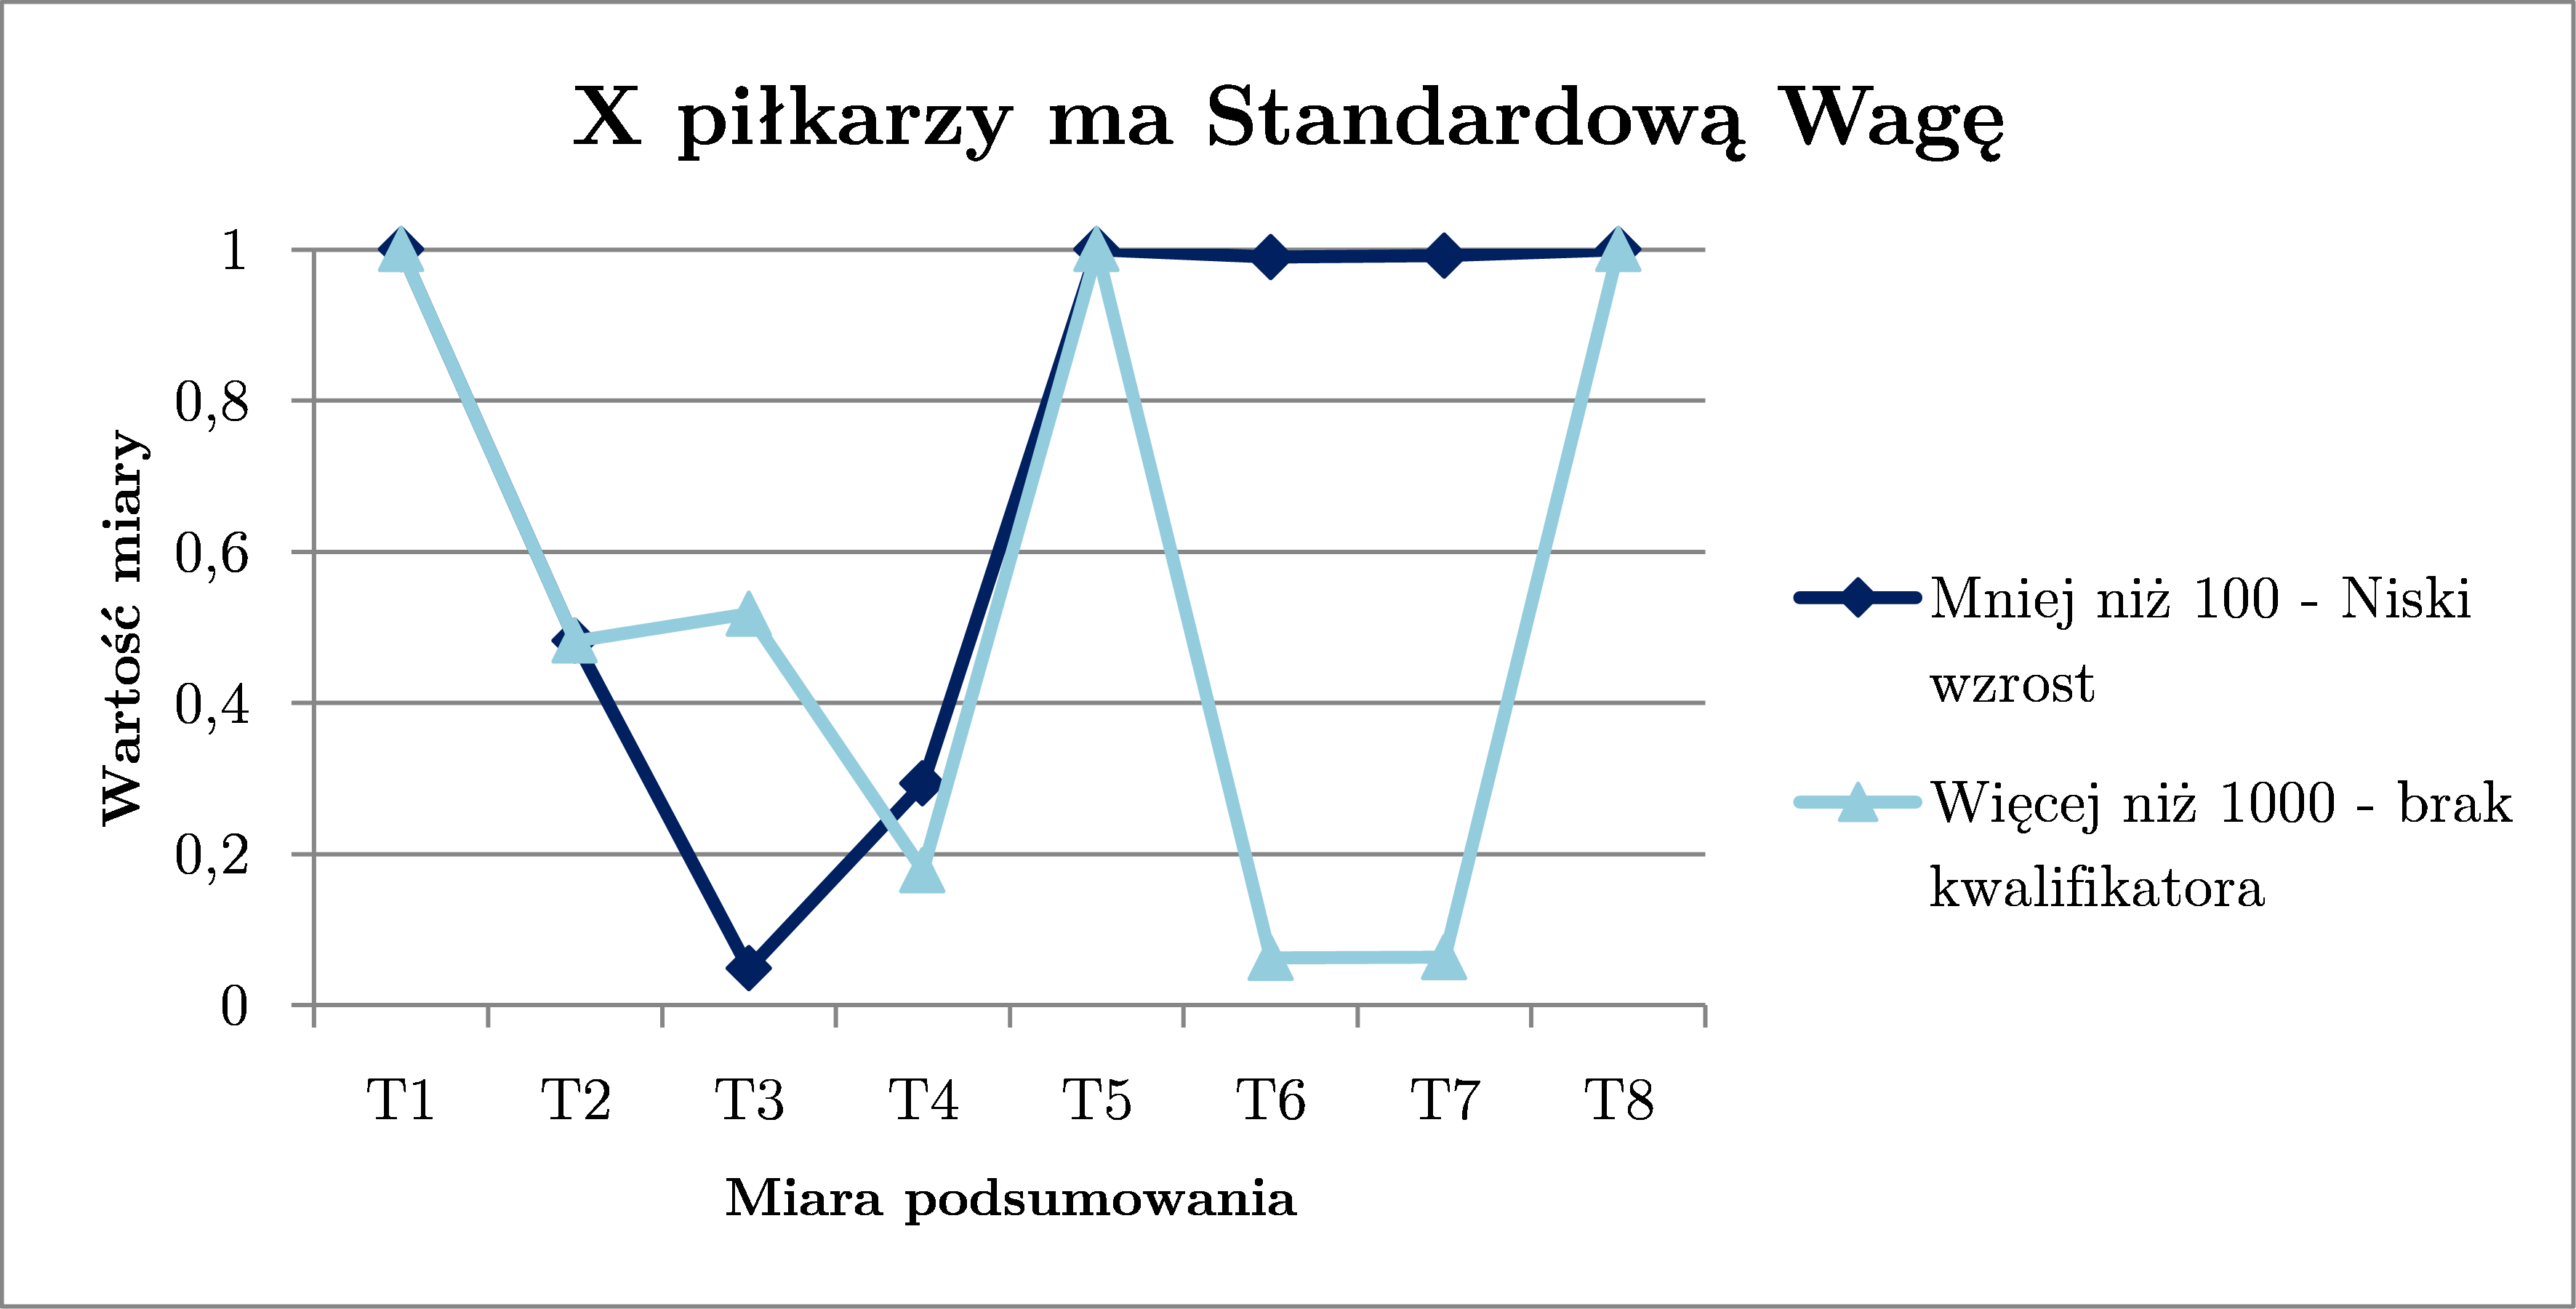
\includegraphics[width=0.9\textwidth]{{Rysunki/Badanie222.png}}
	\caption{Wykres przedstawiający wyniki Eksperymentu 2.2 - kwantyfikator bezwzględny}
\end{figure}

\begin{table}[H]
	\centering
	\begin{tabular}{c c c } 
		\hline
		 & \textbf{Niski Wzrost} & \textbf{Brak kwalifikatora}\\ [0.5ex]
		\textbf{Miara} & \textbf{Mniej niż 100} & \textbf{Więcej niż 1000}\\ [0.5ex]
		\hline
		\hline 
		T1 & 1 & 1 \\
		T2 & 0.482 & 0.482 \\
		T3 & 0.048 & 0.518 \\
		T4 & 0.293 & 0.178 \\
		T5 & 1 & 1 \\
		T6 & 0.99 & 0.062 \\
		T7 & 0.992 & 0.063 \\
		T8 & 1 & 1 \\
		\hline
	\end{tabular}
	\caption{Tabela przedstawiająca wyniki Eksperymentu 2.2 - kwantyfikator bezwzględny}
\end{table}


\subsection{Trzeci eksperyment}

W tym badaniu wygenerowaliśmy komunikaty dotyczących wysokich piłkarzy, którzy mają:
\begin{enumerate}
	\item Słabą Kontrolę,
	\item Słabą Celność,
	\item Słabą Kontrolę ORAZ Słabą Celność,
	\item Słabą Kontrolę LUB Słabą Celność.
\end{enumerate}
Porównywaliśmy zarówno jednakowe, jak i różniące się kwantyfikatory, dla których miara T1 była różna od 0.

\begin{figure}[H]
	\centering
	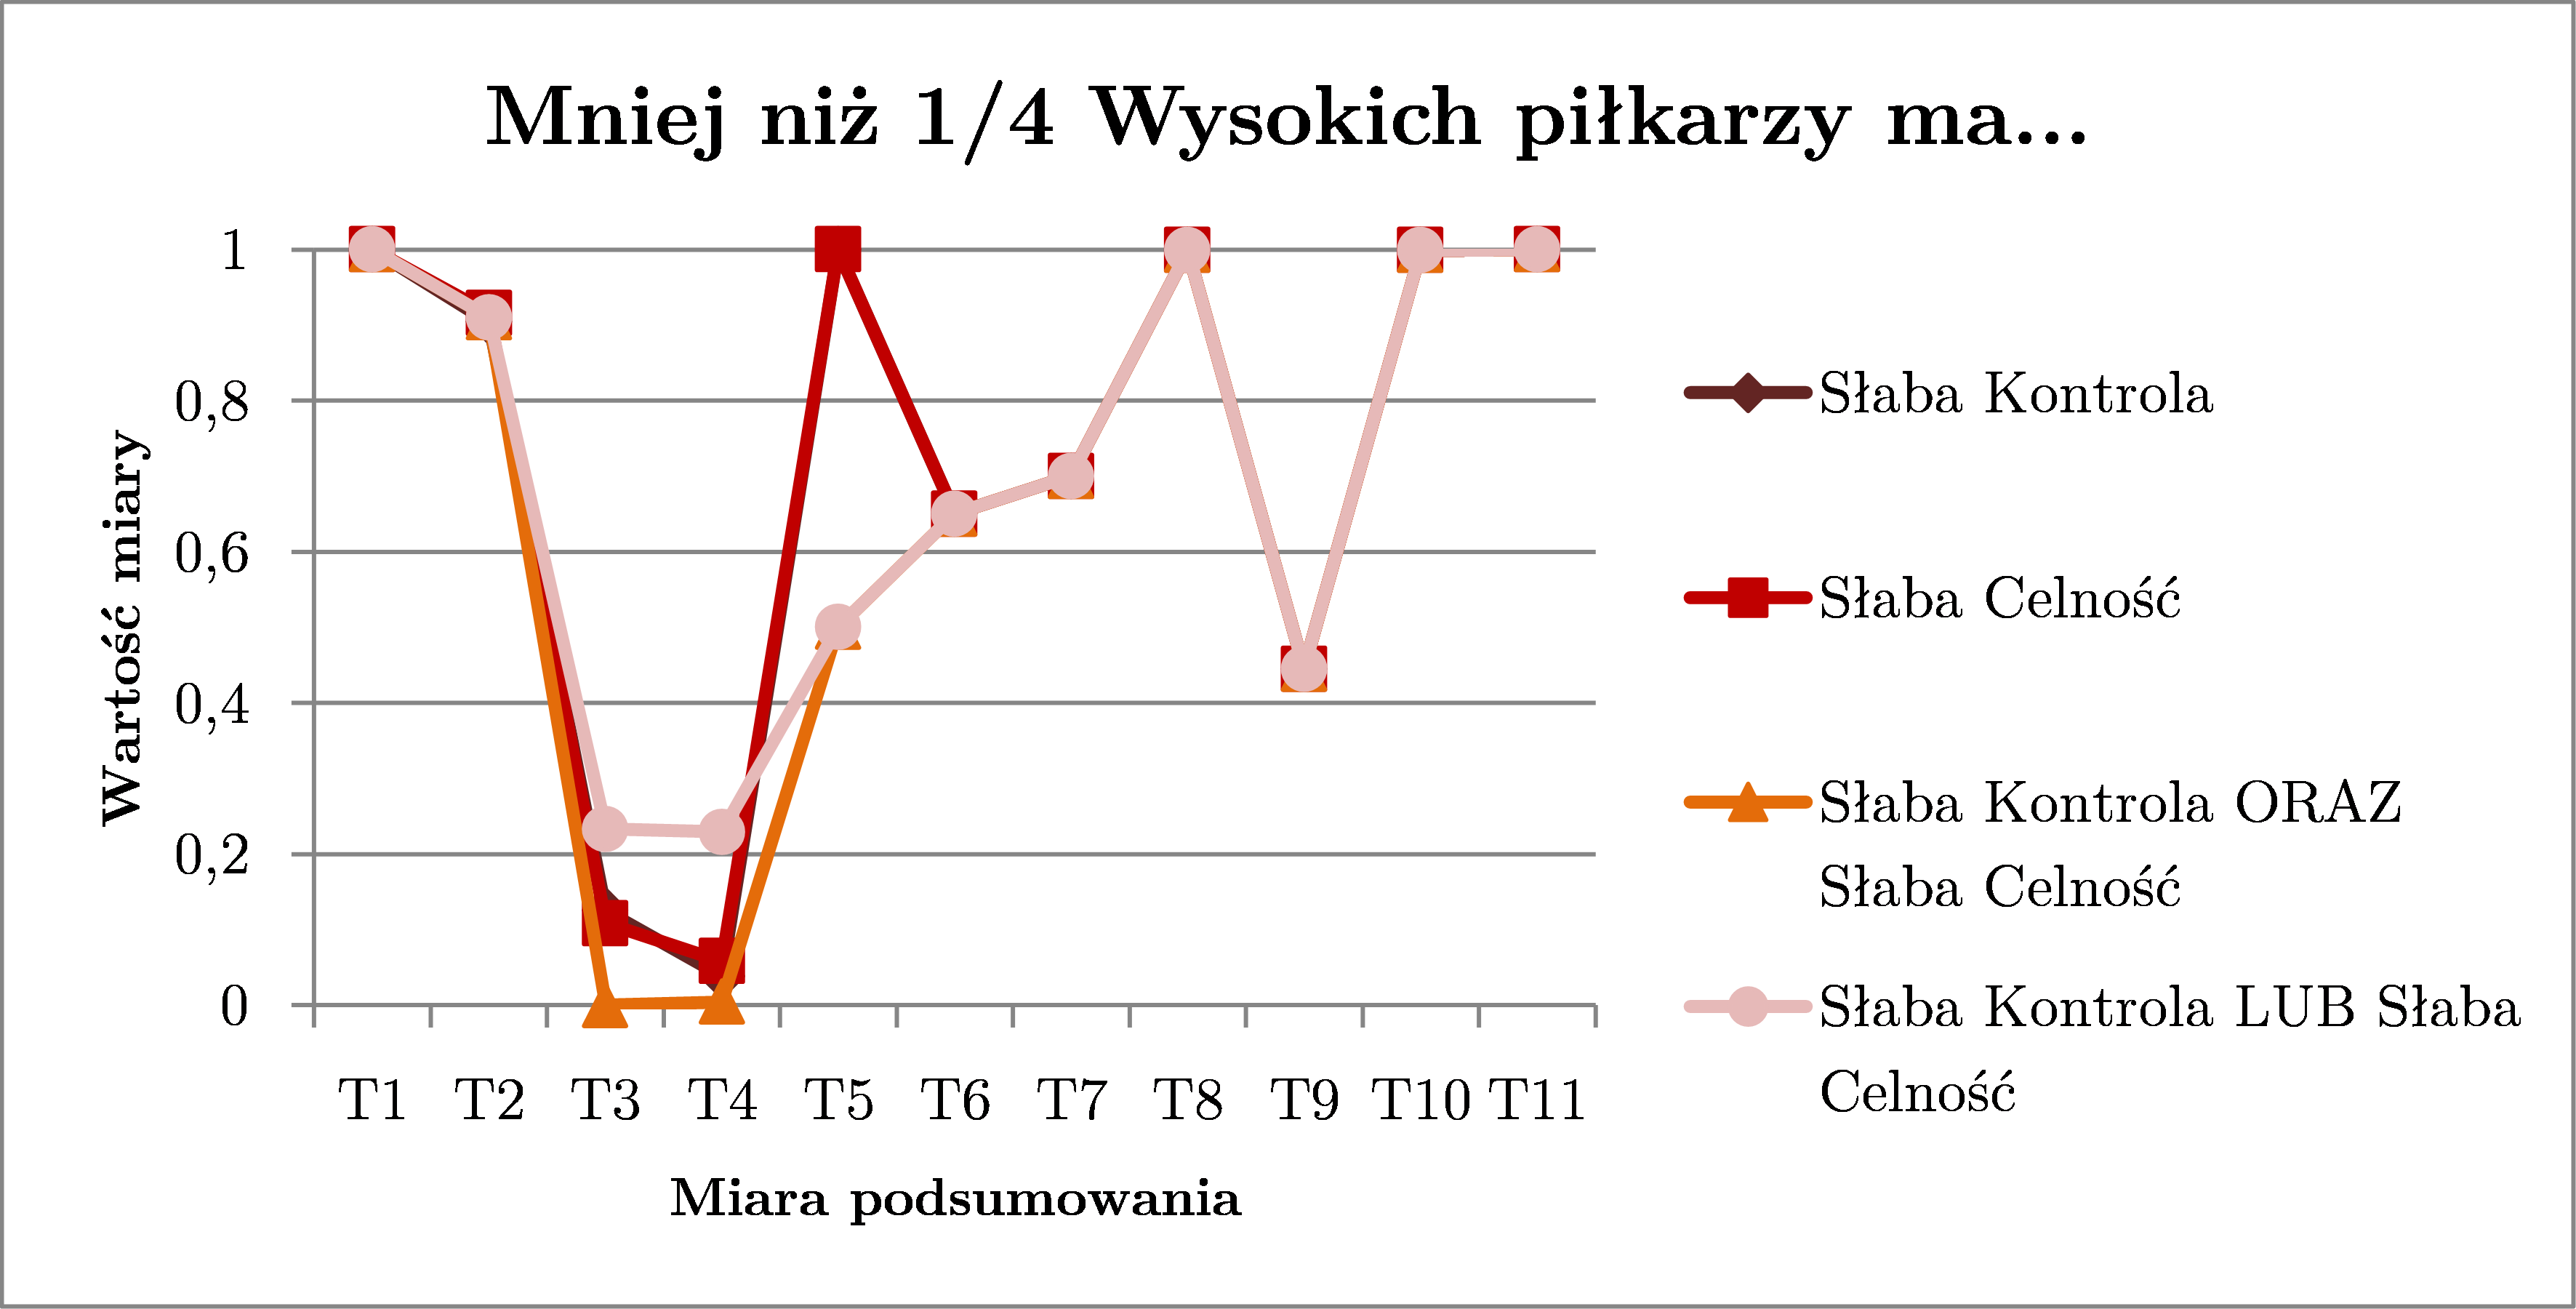
\includegraphics[width=0.9\textwidth]{{Rysunki/Badanie31.png}}
	\caption{Wykres przedstawiający wyniki Eksperymentu 3 - kwantyfikator względny}
\end{figure}

\begin{table}[H]
	\centering
	\begin{tabular}{c c c c c } 
		\hline
		\textbf{Miara} & \textbf{Słaba Kontrola} & \textbf{Słaba Celność} & \textbf{ORAZ} & \textbf{LUB}\\ [0.5ex] 
		\hline
		\hline 
		T1 & 1 & 1 & 1 & 1 \\
		T2 & 0.904 & 0.916 & 0 & 0 \\
		T3 & 0.125 & 0.108 & 0 & 0.233 \\
		T4 & 0.038 & 0.058 & 0.04 & 0.027 \\
		T5 & 1 & 1 & 0.5 & 0.5 \\
		T6 & 0.065 & 0.065 & 0.65 & 0.65 \\
		T7 & 0.7 & 0.7 & 0.7 & 0.7 \\
		T8 & 0.999 & 0.999 & 0.999 & 0.999 \\
		T9 & 0.445 & 0.445 & 0.445 & 0.445 \\
		T10 & 0.999 & 0.999 & 0.999 & 0.999 \\
		T11 & 1 & 1 & 1 & 1 \\
		\hline
	\end{tabular}
	\caption{Tabela przedstawiająca wyniki Eksperymentu 3 - kwantyfikator względny (mniej niż 1/4 piłkarzy)}
\end{table}

\begin{figure}[H]
	\centering
	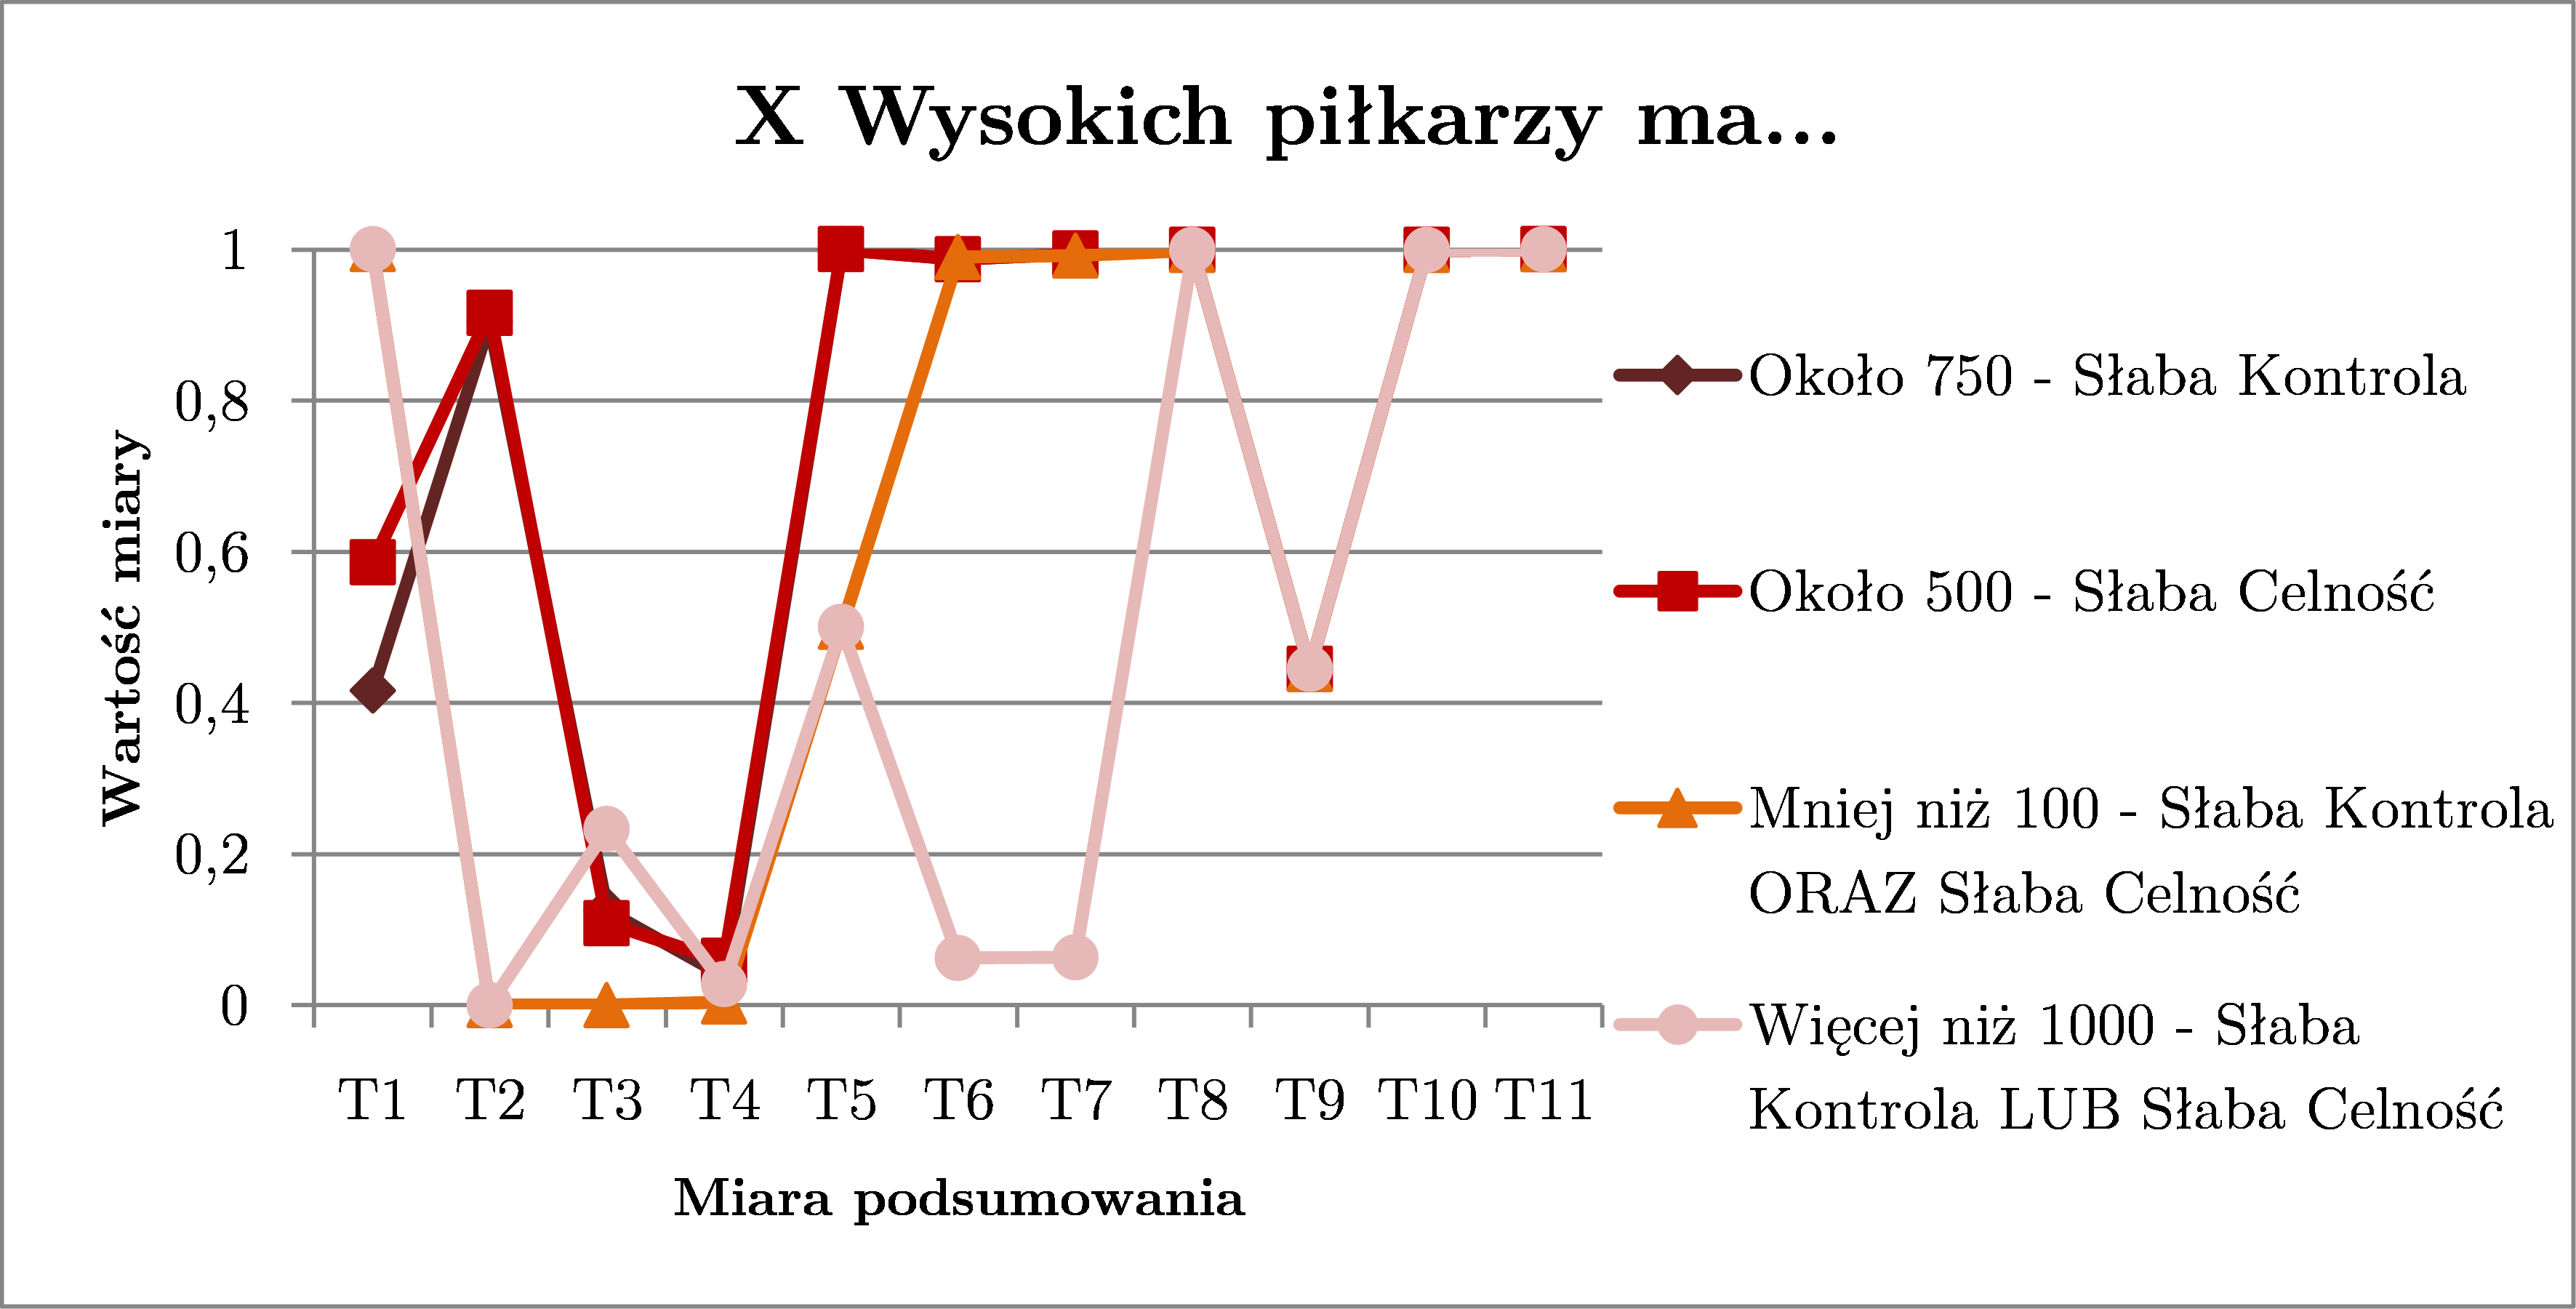
\includegraphics[width=0.9\textwidth]{{Rysunki/Badanie32.png}}
	\caption{Wykres przedstawiający wyniki Eksperymentu 3 - kwantyfikator bezwzględny}
\end{figure}


\begin{table}[H]
	\centering
	\begin{tabular}{c c c c c } 
		\hline
		& \textbf{Słaba Kontrola} & \textbf{Słaba Celność} & \textbf{ORAZ} & \textbf{LUB}\\ [0.5ex] 
		\textbf{Miara} & \textbf{Około 700} & \textbf{Około 500} & \textbf{Mniej niż 100} & \textbf{Więcej niż 1000}\\ [0.5ex] 
		\hline
		\hline 
		T1 & 0.416 & 0.586 & 1 & 1 \\
		T2 & 0.904 & 0.916 & 0 & 0 \\
		T3 & 0.125 & 0.108 & 0 & 0.233 \\
		T4 & 0.038 & 0.058 & 0.04 & 0.027 \\
		T5 & 1 & 1 & 0.5 & 0.5 \\
		T6 & 0.987 & 0.987 & 0.99 & 0.062 \\
		T7 & 0.994 & 0.994 & 0.992 & 0.063 \\
		T8 & 0.999 & 0.999 & 0.999 & 0.999 \\
		T9 & 0.445 & 0.445 & 0.445 & 0.445 \\
		T10 & 0.999 & 0.999 & 0.999 & 0.999 \\
		T11 & 1 & 1 & 1 & 1 \\
		\hline
	\end{tabular}
	\caption{Tabela przedstawiająca wyniki Eksperymentu 3 - kwantyfikator bezwzględny}
\end{table}

\section{Dyskusja}

\subsection{Wpływ kwantyfikatora na miary}

Miara $T1$, obrazująca prawdziwość danego podsumowania, zmieniała się wraz z rozważanym kwantyfikatorem - dla większości będąc równa 0. Obrazuje ona nie tylko jak dużo piłkarzy spełnia dane kryterium, ale pozwala też szacować jak duża jest grupa, która podsumowanej cechy nie spełnia. Dla eksperymentu 1.1 widać jak mało jest piłkarzy którzy posiadając Dobrą Celność, cechują się też Przeciętnym Ustawianiem się. Piłkarze cechujący się Słabą Prędkością w dużej części posiadają Zadowalające Opanowanie - $T1$ jest niskie dla miar około $1/2$ oraz około $2/3$, dzięki czemu wiemy, że właściwa grupa byłaby opisana kwantyfikatorem zawierającym się w przedziale ($\frac{1}{2}$, $\frac{2}{3}$). Liczba ta oscyluje wokół 250 piłkarzy. Sprawa wygląda inaczej dla Młodych piłkarzy - około 1/3 z nich ma Dobrą Prędkość, jednak tym razem jest to ponad 1000 piłkarzy. 
\newline

Miary $T6$ i $T7$ opisują sam kwantyfikator, a dokładnie jego precyzyjność. Wyraźnie widać, że miara mniej niż 1/4 opisuje większy zbiór niż reszta zaproponowanych przez nas kwantyfikatorów względnych. Bardzo nieprecyzyjny jest kwantyfikator bezwzględny więcej niż 1000. Wartości tych miar są identyczne dla wszystkich podsumowań i zależą tylko od kwantyfikatora.
\newline

Miary $T2-T5$ oraz $T8-T11$ nie zmieniały swoich wartości w zależności od użytego kwantyfikatora, co nie jest zaskakujące, mając na uwadze braku wykorzystania kwantyfikatora w tych wzorach. 

\subsection{Wpływ kwalifikatora na miary}
Ciężko jest porównać miarę $T1$ dla kwalifikatora lub jego braku - pracujemy wtedy na innych zbiorach. Wartości dla kwantyfikatorów względnych mogą się zmienić nieznacznie bądź drastycznie. Prawie na pewno zmienią się wartości dla kwantyfikatorów bezwzględnych (zakładając, że są odpowiednio zdefiniowane). Porównując wyniki skupiliśmy się tylko na tych, gdzie wartości miary $T1$ były większe od zera, przez co miary $T6$ i $T7$ potrafią się różnić, co jednak nie ma nic wspólnego z kwalifikatorem.
\newline

Miara $T3$ mówi nam o tym, jak bardzo nośnik kwalifikatora pokrywają się z nośnikiem sumaryzatora. Im wyższa wartość jest tej cechy, tym kwalifikator i sumaryzator są ze sobą mniej powiązane. Zarówno Słaby Balans jak i brak kwalifikatora są mocno powiązane z Przeciętnymi Reakcjami, nie można jednak tego powiedzieć o Standardowej Wadze oraz braku kwalifikatora. Prawie w ogóle nie są ze sobą powiązane Niski Wzrost oraz Standardowa Waga (o czym także mówi kwantyfikator mniej niż 100, dla którego miara T1 jest równa 1). Im wyższa jest ta wartość, tym większy jest kwantyfikator.

Miara $T4$ mówi o tym, jak wiele krotek przynależy do sumaryzatora...

Miary $T2, T5$ oraz $T8$ nie zmieniały swoich wartości, gdyż zależą od sumaryzatora, a nie kwalifikatora. 

\subsection{Wpływ sumaryzatora na miary}

Miara $T2$ która opisuje stopień nieprecyzyjności sumaryzatora...

\section{Wnioski}
\begin{itemize}
	\item Należy dobierać precyzyjnie wartości przy funkcjach przynależności, aby uzyskać miarodajne wyniki.
	\item Parametry dla kwantyfikatora absolutnego muszą być precyzyjnie dobrane do typu i rodzaju bazy - baza składająca się z dużej liczby elementów i dużej liczby atrybutów może potrzebować mniejszych wartości. 
	\item Dodatkowy sumaryzator "i" oraz "lub" ma negatywny wpływ na wartości miar $T_2$ - $T_5$.
	\item Dodatkowy sumaryzator "lub" osiąga wyższe wartości miar, niż sumaryzator "i"
	\item Z powodu braku dodatkowych kwalifikatorów w naszym projekcie, miara $T_11$ nie dostarcza istotnych informacji
	\item Miara $T_1$ zazwyczaj wystarcza do rozstrzygnięcia, które podsumowanie jest lepsze
\end{itemize}

	

\begin{thebibliography}{}
\bibitem{adam}
Methods for the linguistic summarization of data - aplications of fuzzy sets and their extensions, Adam Niewiadomski, Akademicka Oficyna Wydawnicza EXIT, Warszawa 2008
\bibitem{ZbiorRozmyty}
http://www.cs.put.poznan.pl/amichalski/si.dzienne/AI7.new.fuzzy.b\&w.pdf
\bibitem{FunkcjaPrzynaleznosci}
http://home.agh.edu.pl/~mrzyglod/iw/iw\_pliki/iw-is-L2-2017-2018.pdf
\bibitem{BazaDanych}
https://www.kaggle.com/aishwarya1992/fifa-19-player-database
\end{thebibliography}
\end{document}
